
\chapter{Additional experimental results\label{chap:Experimental-results} }

\addcontentsline{lof}{chapter}{Experimental results\lofpost}  
\addcontentsline{lot}{chapter}{Experimental results\lofpost}

\singlespacing 
\epigraph{
A strong claim of violation [of Bell's inequality] should be supported by at least a 5 sigma deviation.}
{Alain Aspect\\Rosenthal Lecture, 2018} 
\doublespacing\noindent \noindent\lettrine{T}{his} chapter presents experimental results
and control experiments that support the main experimental results
and conclusions presented in Chapter~\ref{chap:Introduction-and-overview}.
The characterization of the Hamiltonian parameters, coherence properties,
and other non-idealities of the two-transmon, one-readout-cavity device
employed in the experiment is discussed in Sec.~\ref{sec:Characterization-of-the}.
The calibration  of the tomography and control pulses and relevant
control experiments are discussed in Sec.~\ref{sec:Control-of-the}.
A summary of the  drive amplitudes and frequencies can be found in
Sec.~\ref{subsec:Atom-and-cavity}. Details of the experimental flow
of the catch and reverse protocol with regard to the FPGA controller
are discussed in Sec.~\ref{sec:Catching-and-reversing}. A comparison
between the predictions of the quantum trajectory description of the
experiment developed in Chapter~\ref{chap:theoretical-description-jumps}
and the main experimental results is presented in Sec.~\ref{subsec:Comparison-between-theory}.

\section{Characterization of the system\label{sec:Characterization-of-the}}

In this section, we describe the characterization of the Hamiltonian
and coherence parameters of the two-transmon, one-readout-cavity device
employed in the experiment. In reference to the protected Dark level,
which is engineered to be decoupled from the environment and readout
cavity, we  nickname the device ``Darkmon.''  The low-excitation
manifold of the Darkmon device is well described by the approximate
dispersive Hamiltonian, see Sec.~\ref{sec:circuit-design}, 
\begin{align}
\hat{H}/\hbar= & \omega_{\mathrm{B}}\hat{b}^{\dagger}\hat{b}-\frac{1}{2}\alpha_{\mathrm{B}}\hat{b}^{\dagger2}\hat{b}^{2}+\omega_{\mathrm{D}}\hat{d}^{\dagger}\hat{d}-\frac{1}{2}\alpha_{\mathrm{D}}\hat{d}^{\dagger2}\hat{d}^{2}-\chi_{\mathrm{DB}}\hat{b}^{\dagger}\hat{b}\hat{d}^{\dagger}\hat{d}\label{eq:Hamiltonian-of-sys}\\
 & \left(\omega_{\mathrm{C}}+\chi_{\mathrm{B}}\hat{b}^{\dagger}\hat{b}+\chi_{\mathrm{D}}\hat{d}^{\dagger}\hat{d}\right)\hat{c}^{\dagger}\hat{c}\,,\nonumber 
\end{align}
where $\omega_{\mathrm{D,B,C}}$ are the Dark, Bright, and cavity
mode frequencies, $\hat{d}$, $\hat{b},$ $\hat{c}$ are the respective
mode amplitude (annihilation) operators, $\alpha_{{\rm D}}$ ($\alpha_{{\rm B}}$)
is the Dark (Bright) transmon anharmonicity, $\chi_{\mathrm{D}}$
($\chi_{\mathrm{B}}$) is the dispersive shift between the Dark (Bright)
transmon and the readout cavity, and $\chi_{\mathrm{DB}}$ is the
dispersive shift between the two qubits. The Dark, $\ket{\mathrm{D}}$,
and Bright, $\B,$ states correspond to a single excitation in the
Dark and Bright transmon modes, $\hat{d}^{\dagger}\ket0$ and $\hat{b}^{\dagger}\ket0$,
respectively; see Fig.~\ref{fig:Darkmon-energy-level-diagram} for
a level diagram of the low-energy manifold. 

The readout cavity frequency was spectroscopically measured in reflection
\citep{Geerlings2013}, $\omega_{\mathrm{C}}/2\pi=8979.640\text{\,MHz}$,
and the extracted cavity linewidth agreed well with an independent
measurement of the energy-relaxation rate of the cavity extracted
from a time-domain ring-down measurement, $\kappa/2\pi=3.62\pm0.05\,\mathrm{MHz}.$
The cavity was observed to be well over-coupled; i.e., the coupling
quality factor, $Q_{c}$, dominated the internal quality factor, $Q_{i}$;
making it difficult to precisely extract $Q_{i}.$ The frequency and
anharmonicity of the B transmon were $\omega_{\mathrm{B}}/2\pi=5570.349\,\mathrm{MHz}$
and $\alpha_{\mathrm{B}}/2\pi=195\,\mathrm{MHz}$, respectively, measured
with two-tone pulsed spectroscopy \citep{Geerlings2013,Reagor2016}.
The frequency and anharmonicity of the D transmon, $\omega_{\mathrm{D}}/2\pi=4845.255\,\mathrm{MHz}$
and $\alpha_{\mathrm{D}}/2\pi=152\,\mathrm{MHz}$, respectively, were
measured in a modified two-tone spectroscopy sequence, where the $\G$
level was mapped to the $\B$ level at the end of the spectroscopy
sequence, before the readout, with $\pi$-pulse on the BG transition.
In a similar two-tone spectroscopy experiment, which included a pre-rotation
on either the BG or DG transition, and a measurement rotation after
the probe tone is turned off but before the readout tone is actuated,
the cross-Kerr coupling between the two qubits was measured to be
$\chi_{\mathrm{DB}}/2\pi=61\pm2\,\mathrm{MHz}$. In a standard energy-relaxation
experiment \citep{Geerlings2013}, the $\ket{\mathrm{B}}$ lifetime
was measured to be $T_{\mathrm{1}}^{\mathrm{B}}=28\pm2\,\mathrm{\mu s}$,
which we believe is limited by the Purcell effect with the readout
cavity mode, based on a finite-element calculation, see Sec.~\ref{subsec:Calculation-of-EPR}.
The Ramsey coherence time of $\B$ was $T_{\mathrm{2}}^{\mathrm{R,B}}=18\pm1\,\mathrm{\mu s}$,
possibly limited by photon shot noise \citep{Gambetta2006-dephasing,Rigetti2012}.
The measured Hamiltonian and coherence parameters of the device are
summarized in Table~\ref{tab:system-params}, where the drive parameters
employed in the experiment can also be found. 

\begin{table}
\begin{centering}
\renewcommand*\arraystretch{1.5}
\hspace*{-1.2cm} % manually align to center of page 
\begin{tabular}{rl|rl|rl}
\multicolumn{2}{c|}{\textbf{Readout cavity}} & \multicolumn{2}{c|}{\textbf{BG transition}} & \multicolumn{2}{c}{\textbf{DG transition}}\tabularnewline
\hline 
\hline 
\multicolumn{6}{c}{\textbf{\rule{0pt}{5ex}Mode frequencies and non-linear parameters}}\tabularnewline
\hline 
\textbf{\rule{0pt}{4ex}}$\omega_{\mathrm{C}}/2\pi=$ & $8979.640\text{\,MHz}$ & ~$\omega_{\mathrm{BG}}/2\pi=$ & $5570.349\text{\,MHz}$ & ~$\omega_{\mathrm{DG}}/2\pi=$ & $4845.255\text{\,MHz}$\tabularnewline
 &  & $\chi_{\mathrm{B}}/2\pi=$ & $-5.08\pm0.2\,\mathrm{MHz}$~ & $\chi_{\mathrm{D}}/2\pi=$ & $-0.33\pm0.08\,\mathrm{MHz}$\tabularnewline
 &  & $\alpha_{\mathrm{B}}/2\pi=$ & $195\pm2\,\mathrm{MHz}$ & $\alpha_{\mathrm{D}}/2\pi=$ & $152\pm2\,\mathrm{MHz}$\tabularnewline
 &  & \multicolumn{4}{c}{$\chi_{\mathrm{DB}}/2\pi=61\pm2\,\mathrm{MHz}$}\tabularnewline
\multicolumn{6}{c}{\textbf{\rule{0pt}{5ex}Coherence related parameters}}\tabularnewline
\hline 
\textbf{\rule{0pt}{5ex}}$\kappa/2\pi$= & $3.62\pm0.05\,\mathrm{MHz}$ & $T_{\mathrm{1}}^{\mathrm{B}}=$ & $28\pm2\,\mathrm{\mu s}$ & $T_{\mathrm{1}}^{\mathrm{D}}=$ & $116\pm5\,\mathrm{\mu s}$\tabularnewline
$\eta=$ & $0.33\pm0.03$ & $T_{\mathrm{2\mathrm{R}}}^{\mathrm{B}}=$ & $18\pm1\,\mathrm{\mu s}$ & $T_{\mathrm{2\mathrm{R}}}^{\mathrm{D}}=$ & $120\pm5\,\mathrm{\mu s}$\tabularnewline
$T_{\mathrm{int}}=$ & $260.0\,\mathrm{ns}$ & $T_{\mathrm{2\mathrm{E}}}^{\mathrm{B}}=$ & $25\pm2\,\mathrm{\mu s}$ & $T_{\mathrm{2\mathrm{E}}}^{\mathrm{D}}=$ & $162\pm6\,\mathrm{\mu s}$\tabularnewline
$n_{\mathrm{th}}^{\mathrm{C}}\le$ & $0.0017\pm0.0002$ & $n_{\mathrm{th}}^{\mathrm{B}}\le$ & $0.01\pm0.005$ & $n_{\mathrm{th}}^{\mathrm{D}}\leq$ & $0.05\pm0.01$\tabularnewline
\multicolumn{6}{c}{\textbf{\rule{0pt}{5ex}Drive amplitude and detuning parameters}}\tabularnewline
\hline 
\textbf{\rule{0pt}{5ex}}$\bar{n}=$ & $5.0\pm0.2$ & ~$\Omega_{\mathrm{B}0}/2\pi=$ & $1.20\pm0.01\,\mathrm{MHz}$ & ~$\Omega_{\mathrm{DG}}/2\pi=$ & $20\pm2\,\mathrm{kHz}$\tabularnewline
 &  & ~$\Omega_{\mathrm{B}1}/2\pi=$ & $0.60\pm0.01\,\mathrm{MHz}$ &  & \tabularnewline
$\Delta_{\mathrm{R}}=$ & $\chi_{\mathrm{B}}$ & ~$\Delta_{\mathrm{B}1}/2\pi=$ & $-30.0\,\text{MHz}$ & ~$\Delta_{\mathrm{DG}}/2\pi=$ & $-275.0\,\text{kHz}$\tabularnewline
\end{tabular}
\par\end{centering}
\caption[Compilation of experimental parameters]{\textbf{\label{tab:system-params}Compilation of  experimental parameters.}}
\end{table}


\subsection{Measurement-induced relaxation\textit{ $T_{1}(\bar{n})$\label{subsec:Measurement-induced-relaxation}}}

It has been established in the superconducting qubit community \citep{Boissonneault2009-Photon-induced-relax,Slichter2012,Sank2016-T1vsNbar,Slichter2016-T1vsNbar}
that as a function of the number of photons circulating in the readout
cavity, $\bar{n},$ the energy-relaxation time, $T_{1}$, of a dispersively
coupled qubit is degraded. In Fig.~\ref{fig:T1-vs-nbar}, we show
a measurement of the $T_{1}$ lifetime of the $\B$ and $\D$ states
as a function of the readout drive strength, in units of the number
of circulating photons, $\bar{n}$, when the drive is resonant; the
measurement protocol is explained in the figure caption. As typically
observed in cQED experiments, the Bright level, which is directly
coupled to the readout cavity, exhibits a large parasitic measurement-induced
energy relaxation, $T_{1}^{\mathrm{B}}\left(\bar{n}\right)$ -- its
lifetime suffers more than an order of magnitude degradation. On the
other hand, perhaps surprisingly, the lifetime, $T_{1}^{\mathrm{D}},$
of the Dark state, $\ket{\mathrm{D}}$, remains essentially unaffected,
even at very large drive strengths, $\bar{n}\approx50$. In this sense,
the Dark level is protected from the $T_{1}\left(\bar{n}\right)$
parasitic effect.

\begin{figure}
\begin{centering}
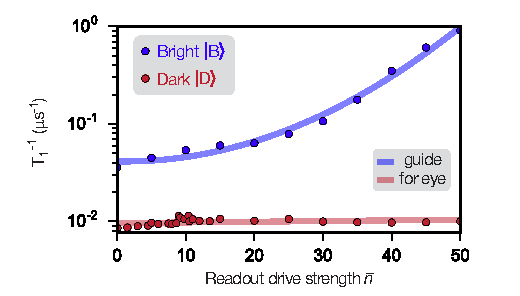
\includegraphics[scale=1.5]{results/T1-vs-nbar}
\par\end{centering}
\caption[Measurement-induced energy relaxation $T_{1}(\bar{n})$]{\label{fig:T1-vs-nbar}\textbf{Measurement-induced energy relaxation
$T_{1}(\bar{n})$.} Energy relaxation rate ($T_{1}^{-1}$) of $\ket{\mathrm{B}}$
(blue dots) and $\ket{\mathrm{D}}$ (red dots) as a function of $\bar{n}$,
measured with the following protocol: after the atom is prepared in
either $\ket{\mathrm{B}}$ or $\ket{\mathrm{D}}$, the readout tone
($\mathrm{R}$) is turned on for duration $t_{\mathrm{read}}$ with
amplitude $\bar{n}$ (corresponding to the number of steady-state
photons in the readout cavity when excited on resonance), whereafter,
the population of the initial state is measured. As in all other experiments,
the readout drive is applied at the $\ket{\mathrm{B}}$ cavity frequency
($\omega_{\mathrm{C}}-\chi_{\mathrm{B}}$). The relaxation rates are
extracted from exponential fits of the population decay as a function
of $t_{\mathrm{read}}$, from $1.3\times10^{7}$ experimental realizations.
The solids lines are guides to the eye: blue line indicates the rapid
degradation of $T_{1}^{\mathrm{B}}$ as a function of the readout
strength, while the red line indicates the nearly constants $T_{1}^{\mathrm{D}}$
of the protected dark level.}
\end{figure}


\section{Control of the three-level atom\label{sec:Control-of-the}}

\subsection{Qubit pulses\label{subsec:Qubit-pulses-calib}}

The implementation of precise and coherent manipulation of the three-level
atom is important for the tomographic reconstruction of the flight
of the quantum jump as well the ability to faithfully reverse it.
One of the main sources of pulse infidelity is typically decoherence,
but the rather long coherence time of the Darkmon device relative
to the duration of the pulses employed in the experiment make it largely
unimportant, and instead, place emphasis on the technical details
of pulse generation and Hamiltonian non-idealities, such as leakage
to higher excited states. 

Mitigation of main technical non-idealities. The effect of the zero-order
hold of the FPGA digital-to-analog converter (DAC) was mitigated by
installing a 270~MHz low pass filter (\textit{Mini-Circuits BLP-300+})
on each of the analog output channels, see Sec.~\ref{sec:Microwave-setup}.
All microwave tones were generated with single-sideband IQ-controlled
modulation at a base intermediate frequency (IF) of 50~MHz, and the
lower radio-frequency (RF) sideband was used for the control tones
(detuned 50~MHz below the local oscillator (LO) frequency). The IQ
mixers were calibrated with a four stage iterative routine to minimize
carrier leakage, by tuning the DC offsets of the I and Q channels,
and to suppress the RF image, by minimizing the quadrature skew and
IQ gain imbalance. The LO leakage could typically be suppressed to
$\approx-70$~dB relative to the RF tone. Spurious intermodulation
tones generated by higher-order non-linear terms present in the mixers
{[}i.e., third-order intercept-point (IP3) products{]} were generally
negligible as the mixers were not typically driven near saturation,
but bandpass filters were installed on the RF outputs of all mixers
to nonetheless suppress any spurious tones. Excess noise from the
following RF amplifier (\textit{MiniCircuits ZVA-183-S+}) was suppressed
by 80\,dB when the control drives were turned off by use of a high-isolation
SPST switch (\textit{Analog Device HMC-C019}).

The pulses applied to the Dark and Bright transition were calibrated
with a combination of Rabi, derivative removal via adiabatic gate
(DRAG) \citep{JChow2010-DRAG}, \emph{All-XY} \citep{Reed2013}, and
amplitude pulse train sequences \citep{Bylander2011}. Pulse timings
and delays, especially between the analog channels and the SPST switch
digital markers, were calibrated with a wide-bandwidth oscilloscope
with ultra-low jitter (\emph{Keysight 86100D Infiniium DCA-X}). The
alignment was verified by performing a Gaussian qubit $\pi$ pulse
on the GB transition and varying the delay between the rise of the
SPST digital marker and the signal on the analog IQ pair playing the
pulse. 


\subsection{Tomography of the three-level atom\label{subsec:Tomography-of-three-level}}

At the end of each experimental realization, we performed one of 15
rotation sequences on the atom that transferred information about
one component of the density matrix, $\hat{\rho}_{a}$, to the population
of $\ket{\mathrm{B}}$, which was measured with a 600~ns square pulse
on the readout cavity. Pulses were calibrated as discussed in Sec.~\ref{subsec:Qubit-pulses-calib}.
The readout signal was demodulated with the appropriate digital filter
function required to realize temporal mode matching \citep{Eichler2012-itinerant-entanglement}.
To remove the effect of potential systematic offset errors in the
readout signal, we subtracted the measurement results of operator
components of $\hat{\rho}_{a}$ and their opposites. From the measurement
results of this protocol, we reconstructed the density matrix $\hat{\rho}_{a}$,
and subsequently parametrized it the useful form 
\begin{equation}
\hat{\rho}_{a}=\begin{pmatrix}\frac{N}{2}\left(1-Z_{\mathrm{GD}}\right) & \frac{N}{2}\left(X_{\mathrm{GD}}+iY_{\mathrm{GD}}\right) & R_{\mathrm{BG}}+iI_{\mathrm{BG}}\\
\frac{N}{2}\left(X_{\mathrm{GD}}-iY_{\mathrm{GD}}\right) & \frac{N}{2}\left(1+Z_{\mathrm{GD}}\right) & R_{\mathrm{BD}}+iI_{\mathrm{BD}}\\
R_{\mathrm{BG}}-iI_{\mathrm{BG}} & R_{\mathrm{BD}}-iI_{\mathrm{BD}} & 1-N
\end{pmatrix},\label{eq:rhoa}
\end{equation}
where $X_{\mathrm{GD}},Y_{\mathrm{GD}},$ and $Z_{\mathrm{GD}}$ are
the Bloch vector components of the GD manifold, $N$ is the total
population of the $\ket{\mathrm{G}}$ and $\ket{\mathrm{D}}$ states,
while $R_{\mathrm{BG}},R_{\mathrm{BD}},I_{\mathrm{BG}}$ and $I_{\mathrm{BD}}$
are the coherences associated with $\ket{\mathrm{B}}$, relative to
the GD manifold. The measured population in $\ket{\mathrm{B}}$, $1-N$,
remains below 0.03 during the quantum jump, see Fig.~\ref{fig:tomo_tmid}.
Tomographic reconstruction was calibrated and verified by preparing
Clifford states, accounting for the readout fidelity of 97\%.

\paragraph{Control experiment.}

In Fig.~\ref{fig:time-resolved-tomo-D}, we show the results of a
control experiment where we verified the Ramsey coherence ($T_{\mathrm{2R}}^{\mathrm{D}}$)
and energy relaxation ($T_{\mathrm{1}}^{\mathrm{D}}$) times of the
DG transition with our tomography method. Solid lines are fitted theoretical
curves for the free evolution of the prepared initial state $\frac{1}{\sqrt{2}}\left(\D-\G\right)$.
The $T_{\mathrm{2R}}^{\mathrm{D}}=119.2\,\mathrm{\mu s}$ value gained
from the simultaneous fit of $X_{\mathrm{DG}}(t)$ and $Y_{\mathrm{DG}}(t)$
matches the lifetime independently obtained from a standard $T_{\mathrm{2R}}$
measurement. Similarly, the value of $T_{\mathrm{1}}^{\mathrm{D}}=115.4\,\mathrm{\mu s}$
extracted from an exponential fit of $Z_{\mathrm{DG}}(t)$ matches
the value obtained from a standard $T_{\mathrm{1}}$ measurement.
We note that our tomography procedure is well calibrated and skew-free,
as evident in the zero steady-state values of $X_{\mathrm{DG}}$ and
$Y_{\mathrm{DG}}$. The steady state $Z_{\mathrm{DG}}$ corresponds
to the thermal population of the dark state $n_{\mathrm{th}}^{\mathrm{D}}$.
It has recently been shown that residual thermal populations in cQED
systems can be significantly reduced by properly thermalizing the
input-output lines \citep{Yeh2017Atten,Wang2019-cav-atten}.

\begin{figure}
\begin{centering}
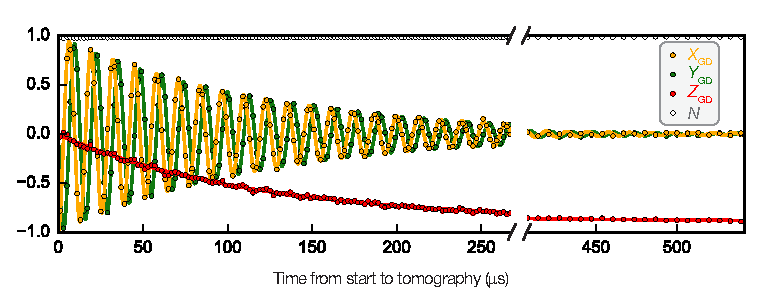
\includegraphics[scale=1.2]{results/time-resolved-tomo-D}
\par\end{centering}
\caption[Control experiment: time-resolved tomogram of the free evolution of
a DG superposition]{\label{fig:time-resolved-tomo-D}\textbf{Control experiment: time-resolved
tomogram of the free evolution of a DG superposition. }The atom is
prepared in $\frac{1}{\sqrt{2}}\left(\D-\G\right)$ and tomography
is performed after a varied delay. Dots: reconstructed conditional
GD tomogram ($X_{\mathrm{DG}},Y_{\mathrm{DG}}$, and $Z_{\mathrm{DG}}$)
and population in DG manifold, $N$, see Eq.~(\ref{eq:rhoa}). Solid
lines: theoretical fits. }
\end{figure}


\paragraph{Mid-flight tomogram.}

In the presence of the coherent Rabi drive $\Odg$ (corresponding
to catch parameter $\Delta t_{\mathrm{off}}=0$), the complete tomogram
of the three-level atom was reconstructed, and a slice at the mid-flight
time, $\Delta t_{\mathrm{mid}}$, is shown in Fig.~\ref{fig:tomo_tmid}.
All imaginary components of the reconstructed conditional density
matrix, $\rho_{\mathrm{c}}$, are negligibly small, less than 0.007,
as expected, see Sec.~\ref{subsec:Comparison-between-theory}, for
well-calibrated tomographic phase control. The population of the $\B$
state, 0.023, is nearly negligible as well, as it is conditioned away
by the IQ filter, see Sec.~\ref{subsec:IQ-filter}.
\begin{figure}
\centering{}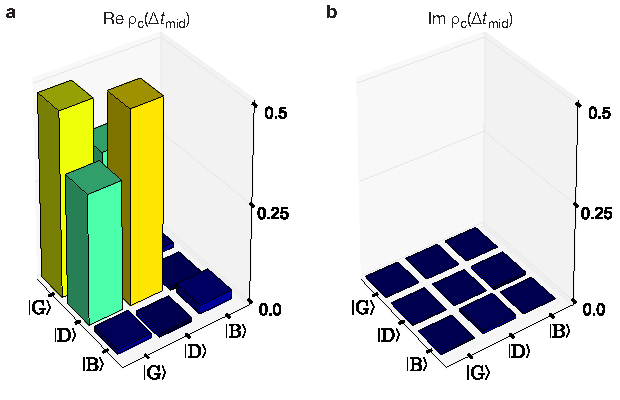
\includegraphics[width=120mm]{results/tomogram_tmid}
\caption[Mid-flight tomogram]{\label{fig:tomo_tmid}\textbf{Mid-flight tomogram. }The plots show
the real (a) and imaginary (b) parts of the conditional density matrix,
$\rho_{\mathrm{c}}$, at the mid flight of the quantum jump ($\Delta t_{\mathrm{catch}}=\Delta t_{\mathrm{mid}}$),
in the presence of the Rabi drive from $\ket{\mathrm{G}}$ to $\ket{\mathrm{D}}$
($\Delta t_{\mathrm{off}}=0$). The population of the $\ket{\mathrm{B}}$
state is 0.023, and the magnitude of all imaginary components is less
than 0.007. }
\end{figure}


\subsection{Atom and cavity drives \label{subsec:Atom-and-cavity}}

In all experiments, unless noted otherwise, the following drive parameters
were used: The DG Rabi drive, $\Omega_{\mathrm{DG}}$, was applied
275~kHz below $\omega_{\mathrm{D}}$ to account for the Stark shift
of the cavity. The BG drive, $\Omega_{\mathrm{BG}}$, was realized
as a bi-chromatic tone in order to unselectively address the BG transition,
which was broadened and Stark shifted due to the coupling between
$\ket{\mathrm{B}}$ and the readout cavity. Specifically, we addressed
transitions from $\ket{\mathrm{G}}$ to $\ket{\mathrm{B}}$ with a
Rabi drive $\Omega_{\mathrm{B0}}/2\pi=1.20\pm0.01\,$~MHz at frequency
$\omega_{\mathrm{BG}}$, whereas transitions from $\ket{\mathrm{B}}$
to $\ket{\mathrm{G}}$ were addressed with a Rabi drive $\Omega_{\mathrm{B1}}/2\pi=0.60\pm0.01\,$~MHz
tuned 30~MHz below $\omega_{\mathrm{BG}}$. This bi-chromatic scheme
provided the ability to tune the up-click and down-click rates independently,
but otherwise essentially functioned as an incoherent broad-band source.
In Table~\ref{tab:Summary-of-timescales.}, we summarize the hierarchy
of timescales established by the drive amplitudes and frequencies
as well as the relevant decoherence properties of the atom.

\begin{table}[!ht]
\begin{centering}
\addtolength{\tabcolsep}{2pt} 
\renewcommand*{\arraystretch}{1.5}
 %
\begin{tabular}{cc>{\raggedright}p{0.65\columnwidth}}
\hline 
\textbf{Symbol}  & \textbf{Value}  & \textbf{Description}\tabularnewline
\hline 
$\Gamma^{-1}$  & $\approx8.8$\,ns  & Effective measurement time of $\ket{\mathrm{B}}$, approximately given
by $1/\kappa\bar{n}$, where $\bar{n}=5\pm0.2$ in the main experiment\tabularnewline
$\kappa^{-1}$  & $44.0\pm0.06$\,ns  & Readout cavity lifetime\tabularnewline
$T_{\mathrm{int}}$  & 260.0\,ns  & Integration time of the measurement record, set in the controller
at the beginning of the experiment \tabularnewline
$\Gamma_{\mathrm{BG}}^{-1}$  & $0.99\pm0.06\,\mathrm{\mu s}$  & Average time the atom rests in $\ket{\mathrm{G}}$ before an excitation
to $\ket{\mathrm{B}}$, see Fig.~\ref{fig:jumps}b\tabularnewline
$\Delta t_{\mathrm{mid}}$  & $3.95\,\mathrm{\mu s}$  & No-click duration for reaching $Z_{\mathrm{GD}}=0$ in the flight
of the quantum jump from $\ket{\mathrm{G}}$ to $\ket{\mathrm{D}}$,
in the full presence of $\Omega_{\mathrm{DG}}$, see Fig.~\ref{fig:catch}b\tabularnewline
$\Gamma_{\mathrm{GD}}^{-1}$  & $30.8\pm0.4\,\mathrm{\mu s}$  & Average time the atom stays in $\ket{\mathrm{D}}$ before returning
to $\ket{\mathrm{G}}$ and being detected, see Fig.~\ref{fig:jumps}b\tabularnewline
$T_{1}^{\mathrm{D}}$  & $116\pm5\,\mathrm{\mu s}$  & Energy relaxation time of $\ket{\mathrm{D}}$\tabularnewline
$T_{2\mathrm{R}}^{\mathrm{D}}$  & $120\pm5\,\mathrm{\mu s}$  & Ramsey coherence time of $\ket{\mathrm{D}}$\tabularnewline
$T_{2\mathrm{E}}^{\mathrm{D}}$  & $162\pm6\,\mathrm{\mu s}$  & Echo coherence time of $\ket{\mathrm{D}}$\tabularnewline
$\Gamma_{\mathrm{DG}}^{-1}$  & $220\pm5\,\mathrm{\mu s}$  & Average time between two consecutive $\ket{\mathrm{G}}$ to $\ket{\mathrm{D}}$
jumps\tabularnewline
\end{tabular}
\par\end{centering}
\caption[Summary of timescales]{\textbf{Summary of timescales. }List of the characteristic timescales
involved in the catch and reverse experiment. The Hamiltonian parameters
of the system are summarized in Sec.~\ref{sec:Characterization-of-the}.
\textbf{\label{tab:Summary-of-timescales.}}}
\end{table}


\section{Monitoring quantum jumps in real time }

\subsection{IQ filter \label{subsec:IQ-filter}}

To mitigate the effects of imperfections in the atom readout scheme
in extracting a $\ket{\mathrm{B}}$/not-$\ket{\mathrm{B}}$ result,
we applied a two-point, hysteretic IQ filter, implemented on the FPGA
controller in real time. The filter is realized by comparing the present
quadrature record values $\left\{ I_{\mathrm{rec}},Q_{\mathrm{rec}}\right\} $,
with three thresholds ($I_{\mathrm{B}},I_{\bar{\mathrm{B}}},$ and
$Q_{\mathrm{B}}$) in the following way: 
\begin{center}
\begin{tabular}{>{\raggedleft}m{20mm}|>{\centering}p{30mm}|>{\centering}p{30mm}|>{\centering}p{30mm}}
\textbf{Input: } & $Q_{\mathrm{rec}}\geq Q_{\mathrm{B}}$ or

$I_{\mathrm{rec}}>I_{\mathrm{B}}$  & $Q_{\mathrm{rec}}<Q_{\mathrm{B}}$ and

$I_{\mathrm{rec}}<I_{\bar{\mathrm{B}}}$  & $Q_{\mathrm{rec}}<Q_{\mathrm{B}}$ and

$I_{\bar{\mathrm{B}}}\leq I_{\mathrm{rec}}\leq I_{\mathrm{B}}$\tabularnewline
\hline 
\textbf{Output: } & $\ket{\mathrm{B}}$  & not-$\ket{\mathrm{B}}$  & previous\tabularnewline
\end{tabular}
\par\end{center}

\noindent The filter and thresholds were selected to provide a best
estimate of the time of a click, operationally understood as a change
in the filter output from $\ket{\mathrm{B}}$ to not-$\ket{\mathrm{B}}$.
The $I_{{\mathrm{B}}}$ and $I_{\bar{\mathrm{B}}}$ thresholds were
chosen 1.5 standard deviations away from the I-quadrature mean of
the $\ket{\mathrm{B}}$ and not-$\ket{\mathrm{B}}$ distributions,
respectively. The $Q_{{\mathrm{B}}}$ threshold was chosen 3 standard
deviations away from the Q-quadrature mean. Higher excited states
of the atom were selected out by $Q_{\mathrm{rec}}$ values exceeding
the $Q_{\mathrm{B}}$ threshold. 

\subsection{Unconditioned monitoring}

In Sec.~\ref{sec:Unconditioned-monitoring-of}, we described a protocol
for the unconditioned monitoring of the quantum jumps where the atom
is subject to the continuous Rabi drives $\Omega_{\mathrm{BG}}$ and
$\Omega_{\mathrm{DG}}$, as depicted in Fig.~\ref{fig:setup}. From
the continuous tracking of the quantum jumps, over 3.2~s. of data,
we histogrammed the times, $\tau_{\operatorname{not-B}}$, spent in
not-$\ket{\mathrm{B}}$, Fig.~\ref{fig:jumps}b. In Fig.~\ref{fig:B-wait-time},
we show the complimentary histogram for the times, $\tau_{{\rm B}},$
spent in $\B$, which is unlike the latter, in that it follows a single
exponential decay law. This single Poisson process character follows
from the fact that the $\B$ measurement result collapses the atom
to a single state, $\B$, unlike the not-$\B$ result. The average
time spent in $\B$, extracted from the fit, is $\bar{\tau}_{{\rm B}}=4.2\pm0.03\,\mathrm{\mu s}$.
\begin{figure}
\centering{}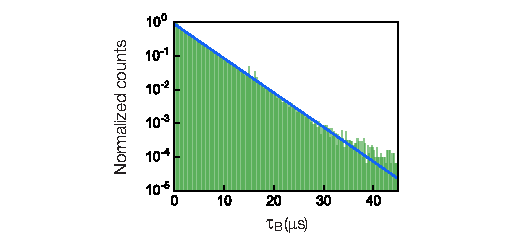
\includegraphics[width=145mm]{results/B_waiting_time}
\caption[Waiting time to switch from a $\B$ to not-$\B$ state assignment
result]{\label{fig:B-wait-time}\textbf{Waiting time to switch from a $\B$
to not-$\B$ state assignment result.} Semi-log plot of the histogram
(shaded green) of the duration of times corresponding to $\B$-measurement
results, $\tau_{\operatorname{B}}$, for 3.2~s of continuous data
of the type shown in Fig.~\ref{fig:jumps}a. Solid line is an exponential
fit, which yields a $4.2\pm0.03\,\mathrm{\mu s}$ time constant. }
\end{figure}

\pagebreak{}

\section{Catching and reversing the jump \label{sec:Catching-and-reversing}}

\subsection{Experiment flow}

\begin{figure}
\begin{centering}
%\hspace*{-1cm} % manually align to center of page 
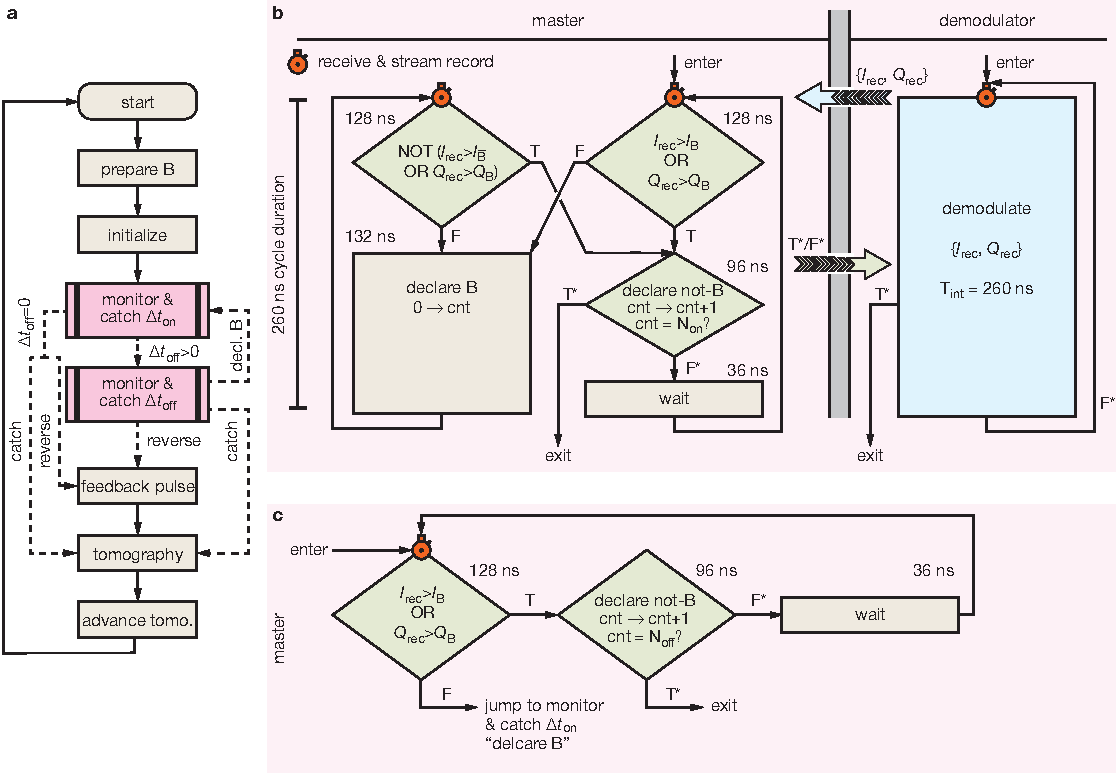
\includegraphics[angle=-90,scale=1.1]{results/experiment_flow}
\par\end{centering}
\caption[Experiment flow]{\label{fig:experiment-flow}\textbf{Experiment flow. }See text for
detailed description.}
\end{figure}
Figure \ref{fig:experiment-flow}a shows a flowchart representation
of steps involved in the catch and reverse protocol. In the following,
we describe each block in the diagram in the order in which it would
be executed.

\paragraph{Start:}

internal memory registers are set to zero \citep{Ofek2016,Liu2016Thesis},
including the no-click counter ``cnt,'' defined below. 

\paragraph{Prepare B:}

controller deterministically prepares the atom in $\ket{\mathrm{B}}$,
a maximally conservative initial state, with measurement-based feedback
\citep{Riste2012-qubit-measure-reset}. 

\paragraph{Initialize:}

controller turns on the atom ($\Omega_{\mathrm{BG}}$ and $\Omega_{\mathrm{DG}}$)
and cavity drives ($\mathrm{R}$) and begins demodulation. 

\paragraph{Monitor and catch $\Delta t_{\mathrm{on}}$: }

with all drives on ($\Omega_{\mathrm{BG}},\Omega_{\mathrm{DG}}$,
and $\mathrm{R}$), the controller actively monitors the cavity output
signal until it detects no-clicks for duration $\Delta t_{\mathrm{on}}$,
as described in panel (b), whereafter, the controller proceeds to
``monitor and catch $\Delta t_{\mathrm{off}}$'' in the case that
$\Delta t_{\mathrm{off}}>0$; otherwise, for $\Delta t_{\mathrm{off}}=0$,
the controller proceeds to ``tomography'' (``feedback pulse'')
for the catch (reverse) protocol.

\paragraph{Monitor and catch $\Delta t_{\mathrm{off}}$: }

with the Rabi drive $\Omega_{\mathrm{DG}}$ off, while keeping the
drives $\Omega_{\mathrm{BG}}$ and R on, the controller continues
to monitor the output signal. The controller exits the routine only
if it detects a click, proceeding to the ``declare B'' step of the
``monitor and catch $\Delta t_{\mathrm{on}}$'' routine, or if no
further clicks are detected for the pre-defined duration $\Delta t_{\mathrm{off}}$,
proceeding to ``tomography'' (``feedback pulse'') for the catch
(reverse) protocol.

\paragraph{Feedback pulse: }

with all the continuous drives turned off, the controller performs
a pulse on the DG transition of the atom, defined by the two angles
$\left\{ \theta_{I}\left(\Delta t_{\mathrm{catch}}\right),\varphi_{I}\left(\Delta t_{\mathrm{catch}}\right)\right\} $.

\paragraph{Tomography: }

controller performs next-in-order tomography sequence (see Sec.~\ref{subsec:Tomography-of-three-level})
while the demodulator finishes processing the final data in its pipeline.

\paragraph{Advance tomo.: }

tomography sequence counter is incremented, and after a $50~\mathrm{\mu s}$
delay, the next realization of the experiment is started.

\subsubsection{Logic and timing of catch subroutines}

\paragraph{Monitor and catch $\Delta t_{\mathrm{on}}$.}

Figure \ref{fig:experiment-flow}b shows a concurrent-programming
flowchart representation of the ``monitor and catch $\Delta t_{\mathrm{on}}$''
routine. Displayed are the master and demodulator modules of the controller.
The demodulator outputs a pair of 16 bit signed integers, $\left\{ I_{\mathrm{rec}},Q_{\mathrm{rec}}\right\} $,
every $T_{\mathrm{int}}=260$~ns, which is routed to the master module,
as depicted by the large left-pointing arrow. The master module implements
the IQ filter (see Sec.~\ref{subsec:IQ-filter}) and tracks the number
of consecutive not-$\ket{\mathrm{B}}$ measurement results with the
counter cnt. The counter thus keeps track of the no-click time elapsed
since the last click, which is understood as a change in the measurement
result from $\ket{\mathrm{B}}$ to not-$\ket{\mathrm{B}}$. When the
counter reaches the critical value $N_{\mathrm{on}}$, corresponding
to $\Delta t_{\mathrm{on}}$, the master and demodulator modules synchronously
exit the current routine, see the T{*} branch of the ``declare not-B''
decision block. Until this condition is fulfilled (F{*}), the two
modules proceed within the current routine as depicted by the black
flowlines. 

To minimize latency and maximize computation throughput, the master
and demodulator were designed to be independent sequential processes
running concurrently on the FPGA controller, communicating strictly
through synchronous message passing, which imposed stringent synchronization
and execution time constraints. All master inter-module logic was
constrained to run at a 260~ns cycle, the start of which necessarily
was imposed to coincide with a ``receive \& stream record'' operation,
here, denoted by the stopwatch. In other words, this imposed the algorithmic
constraint that all flowchart paths staring at a stopwatch and ending
in a stopwatch, itself or other, were constrained to a 260\,ns execution
timing. A second key timing constraint was imposed by the time required
to propagate signals between the different FPGA cards, which corresponded
to a minimum branching-instruction duration of 76~ns.

\paragraph{Monitor and catch $\Delta t_{\mathrm{off}}$.}

Figure \ref{fig:experiment-flow}c shows a concurrent-programming
flowchart representation of the master module of the ``monitor and
catch $\Delta t_{\mathrm{off}}$'' routine. The corresponding demodulation-module
flowchart is identical to that shown of panel (b); hence, it is not
shown. This routine functions in following manner: If a $\ket{\mathrm{B}}$
outcome is detected, the controller jumps to the ``declare B'' block
of the monitor \& catch $\Delta t_{\mathrm{on}}$ routine; otherwise,
when only not-$\ket{\mathrm{B}}$ outcomes are observed, and the counter
reaches the critical value $N_{\mathrm{off}}$, corresponding to $\Delta t_{\mathrm{catch}}=\Delta t_{\mathrm{on}}+\Delta t_{\mathrm{off}}$,
the controller exits the routine.

\section{Comparison between theory and experiment \label{subsec:Comparison-between-theory}\label{subsec:Error-analysis}}

In this section, we present the comparison between the results of
the quantum jumps experiment and the predictions of the quantum trajectory
theory of the experiment developed in Chapter~\ref{chap:theoretical-description-jumps}.
The results agree with the theoretical predictions, accounting for
known imperfections, essentially without adjustable parameters. Simulation
plots courtesy of H.J. Carmichael. 

\subsection{Simulated data sets}

\paragraph{\textit{\emph{Independently measured parameters.}}}

The parameters used in the Monte Carlo simulation described in Sec.~\ref{subsec:Simulation-of-linear}
are listed in Table~\ref{table:table2}. Nearly all are set to the
value at the center of the range quoted in Table~\ref{tab:system-params},
with three exceptions: i) $T_{1}^{{\rm B}}$ and $T_{1}^{{\rm D}}$
are set to lower values in response to the photon number dependence
of the readout displayed in Fig.~\ref{fig:T1-vs-nbar}, ii) $\Omega_{{\rm DG}}/2\pi$
is set higher, but still falls inside the experimental error bars,
and iii) $n_{{\rm th}}^{{\rm C}}=0$. Notably, of the three exceptions,
only $\Omega_{{\rm DG}}/2\pi$ has a noticeable effect on the comparison
between simulated and experimental data sets.

\paragraph{\textit{\emph{Leakage from the }}\emph{GBD}\textit{\emph{-manifold.}}\emph{ }}

As discussed in Sec.~\ref{sec:circuit-design}, see Fig.~\ref{fig:Darkmon-energy-level-diagram},
the Darkmon system has higher excited states, which are generally
unimportant, but do contribute a small imperfection that needs to
be considered to qualitatively account for the results. As discussed
in Sec.~\ref{subsec:Simulation-of-linear}, we model the effect of
leakage from the GBD manifold by adding a single additional higher-excited
state level, denoted $\ket{\mathrm{F}}.$ The additional random jumps
to state $|{\rm F}\rangle$ are governed by four parameters that are
not independently measured; they serve as fitting parameters, required
to bring the simulation into agreement with the asymptotic behavior
of ${\rm Z}(\Delta t_{{\rm catch}})$, which, without leakage to $|{\rm F}\rangle$,
settles to a value higher than is measured in the experiment. The
evolution of the ${\rm X}(\Delta t_{{\rm catch}})$ is largely unaffected
by the assignment of these parameters, where any change that does
occur can be offset by adjusting $\Omega_{{\rm DG}}/2\pi$ while staying
within the experimental error bars.

\paragraph{\textit{\emph{Ensemble average.}}\emph{ }}

Simulated data sets are computed as an ensemble average by sampling
an ongoing Monte Carlo simulation, numerically implementing the model
outlined in Eqs.~(\ref{eqn:SSE_continuous})--(\ref{eqn:jumps_to_F}).
Quadratures $I_{{\rm rec}}$ and $Q_{{\rm rec}}$ are computed from
Eqs.~(\ref{eqn:simulated_I_int}) and (\ref{eqn:simulated_Q_int}),
digitized with integration time $T_{{\rm int}}=260\mkern2mu {\rm ns}$,
and then, as in the experiment, a hysteric filter is used to locate
``click'' events ($\Delta t_{{\rm catch}}=0$) corresponding to
an inferred change of state from $|{\rm B}\rangle$ to not-$|{\rm B}\rangle$.
During the subsequent sampling interval ($\Delta t_{{\rm catch}}\geq0$),
the four quantities 
\begin{equation}
\big({\rm Z}_{{\rm GD}}^{j},{\rm X}_{{\rm GD}}^{j},{\rm Y}_{{\rm GD}}^{j},{\rm P}_{{\rm BB}}^{j}\big)(\Delta t_{{\rm catch}})=\big({\rm Z}_{{\rm GD}}^{{\rm rec}},{\rm X}_{{\rm GD}}^{{\rm rec}},{\rm Y}_{{\rm GD}}^{{\rm rec}},{\rm P}_{{\rm BB}}^{{\rm rec}}\big)(t_{j}+\Delta t_{{\rm catch}}),
\end{equation}
with $t_{j}$ is the click time and 
\begin{eqnarray}
{\rm Z}_{{\rm GD}}^{{\rm rec}}(t) & = & \frac{\langle{\rm D}|\psi(t)\rangle\langle\psi(t)|{\rm D}\rangle-\langle{\rm G}|\psi(t)\rangle\langle\psi(t)|{\rm G}\rangle}{\langle\psi(t)|\psi(t)\rangle},\label{eqn:correlated_Z_GD}\\
\noalign{\vskip4pt}{\rm X}_{{\rm GD}}^{{\rm rec}}(t)+i{\rm Y}_{{\rm GD}}^{{\rm rec}}(t) & = & 2\frac{\langle{\rm D}|\psi(t)\rangle\langle\psi(t)|{\rm G}\rangle}{\langle\psi(t)|\psi(t)\rangle},\label{eqn:correlated_X_GD=000026Y_GD}\\
\noalign{\vskip4pt}{\rm P}_{{\rm BB}}^{{\rm rec}}(t) & = & \frac{\langle{\rm B}|\psi(t)\rangle\langle\psi(t)|{\rm B}\rangle}{\langle\psi(t)|\psi(t)\rangle},
\end{eqnarray}
are computed, and running sums of each are updated. The sample terminates
when the measurement record indicates a change of state from not-$|{\rm B}\rangle$
back to $|{\rm B}\rangle$. Finally, for comparison with the experiment,
Bloch vector components are recovered from the average over sample
intervals via the formula 
\begin{equation}
\big({\rm Z}_{{\rm GD}},{\rm X}_{{\rm GD}},{\rm Y}_{{\rm GD}}\big)(\Delta t_{{\rm catch}})=\frac{\sum_{j}^{N(\Delta t_{{\rm catch}})}\big({\rm Z}_{{\rm GD}}^{j},{\rm X}_{{\rm GD}}^{j},{\rm Y}_{{\rm GD}}^{j}\big)(\Delta t_{{\rm catch}})}{N(\Delta t_{{\rm catch}})-\sum_{j}^{N(\Delta t_{{\rm catch}})}P_{{\rm BB}}^{j}(\Delta t_{{\rm catch}})},\label{eqn:ensemble_average}
\end{equation}
where $N(\Delta t_{{\rm catch}})$ is the number of sample intervals
that extend up to, or beyond, the time $\Delta t_{{\rm catch}}$.
The simulation and sampling procedure is illustrated in Fig.~\ref{fig:monte-carlo},
and a comparison between the experiment and the simulation is provided
in Fig.~\ref{fig:simulation_vs_experiment}.

The simulated and measured Bloch vector components are fit with expressions
motivated by Eqs.~(\ref{eqn:Z_approx})-(\ref{eqn:Y_approx}) and~(\ref{eq:ZGDXGD-long-term}),
modified to account for the effect of non-idealities in the experiment,
\begin{align}
\mathrm{Z}_{\text{GD}}(\Delta t_{\operatorname{catch}}) & =\ensuremath{a+b\tanh(\Delta t_{\operatorname{catch}}/\tau+c)},\\
\ensuremath{\mathrm{X}_{\text{GD}}(\Delta t_{\operatorname{catch}})} & =a'+b'\operatorname{sech}(\Delta t_{\operatorname{catch}}/\tau'+c')\,,\\
\mathrm{Y}_{\text{GD}}(\Delta t_{\operatorname{catch}}) & =0\,.
\end{align}
The fit parameters ($a,a',b,b',c,c',\tau,\tau'$) for the simulated
and experimental data shown in Fig.~\ref{fig:simulation_vs_experiment}
are compared in Table~\ref{tab:Comparison-of-parameters}. As imposed
by Eq.~(\ref{eq:ZGDXGD-long-term}), in the absence of $\Omega_{{\rm DG}}$
(turned off at time $\Delta t_{{\rm on}}=2\mkern2mu \mu{\rm s}$)
$a'$, the offset of $\mathrm{X}_{\text{GD}}$, is strictly enforced
to be zero. The extracted simulation and experiment parameters are
found to agree at the percent level.

\begin{table}[t]
\begin{centering}
\renewcommand*\arraystretch{1.5}
%\hspace*{-1.2cm} % manually align to center of page 
\begin{tabular}{rl|rl|rl}
\multicolumn{2}{c|}{\textbf{Readout cavity}} & \multicolumn{2}{c|}{\textbf{BG transition}} & \multicolumn{2}{c}{\textbf{DG transition}}\tabularnewline
\hline 
\hline 
\multicolumn{6}{c}{\textbf{\rule{0pt}{5ex}Non-linear parameters}}\tabularnewline
\hline 
 &  & $\chi_{\mathrm{B}}/2\pi=$ & $-5.08\,\mathrm{MHz}$~ & $\chi_{\mathrm{D}}/2\pi=$ & $-0.33\,\mathrm{MHz}$\tabularnewline
\multicolumn{6}{c}{\textbf{\rule{0pt}{5ex}Coherence related parameters}}\tabularnewline
\hline 
\textbf{\rule{0pt}{5ex}}$\kappa/2\pi$= & $3.62\mathrm{MHz}$ & $T_{\mathrm{1}}^{\mathrm{B}}=$ & $15\,\mathrm{\mu s}$ & $T_{\mathrm{1}}^{\mathrm{D}}=$ & $105\,\mathrm{\mu s}$\tabularnewline
$\eta=$ & $0.33$ & $T_{\mathrm{2\mathrm{R}}}^{\mathrm{B}}=$ & $18\,\mathrm{\mu s}$ & $T_{\mathrm{2\mathrm{R}}}^{\mathrm{D}}=$ & $120\,\mathrm{\mu s}$\tabularnewline
$T_{\mathrm{int}}=$ & $260.0\,\mathrm{ns}$ &  &  &  & \tabularnewline
$n_{\mathrm{th}}^{\mathrm{C}}=$ & $0$ & $n_{\mathrm{th}}^{\mathrm{B}}=$ & $0.01$ & $n_{\mathrm{th}}^{\mathrm{D}}=$ & $0.05$\tabularnewline
\multicolumn{6}{c}{\textbf{\rule{0pt}{5ex}Drive amplitude and detuning parameters}}\tabularnewline
\hline 
\textbf{\rule{0pt}{5ex}}$\bar{n}=$ & $5.0$ & ~$\Omega_{\mathrm{B}0}/2\pi=$ & $1.20\,\mathrm{MHz}$ & ~$\Omega_{\mathrm{DG}}/2\pi=$ & $21.6\,\mathrm{kHz}$\tabularnewline
 &  & ~$\Omega_{\mathrm{B}1}/2\pi=$ & $0.60\,\mathrm{MHz}$ &  & \tabularnewline
$\Delta_{\mathrm{R}}=$ & $\chi_{\mathrm{B}}$ & ~$\Delta_{\mathrm{B}1}/2\pi=$ & $-30.0\,\text{MHz}$ & ~$\Delta_{\mathrm{DG}}/2\pi=$ & $-274.5\,\text{kHz}$\tabularnewline
\end{tabular}
\par\end{centering}
\caption[Compilation of the simulation parameters]{\textbf{Compilation of the simulation parameters.}}
\label{table:table2} 
\end{table}

\begin{figure}[t]
\centering{}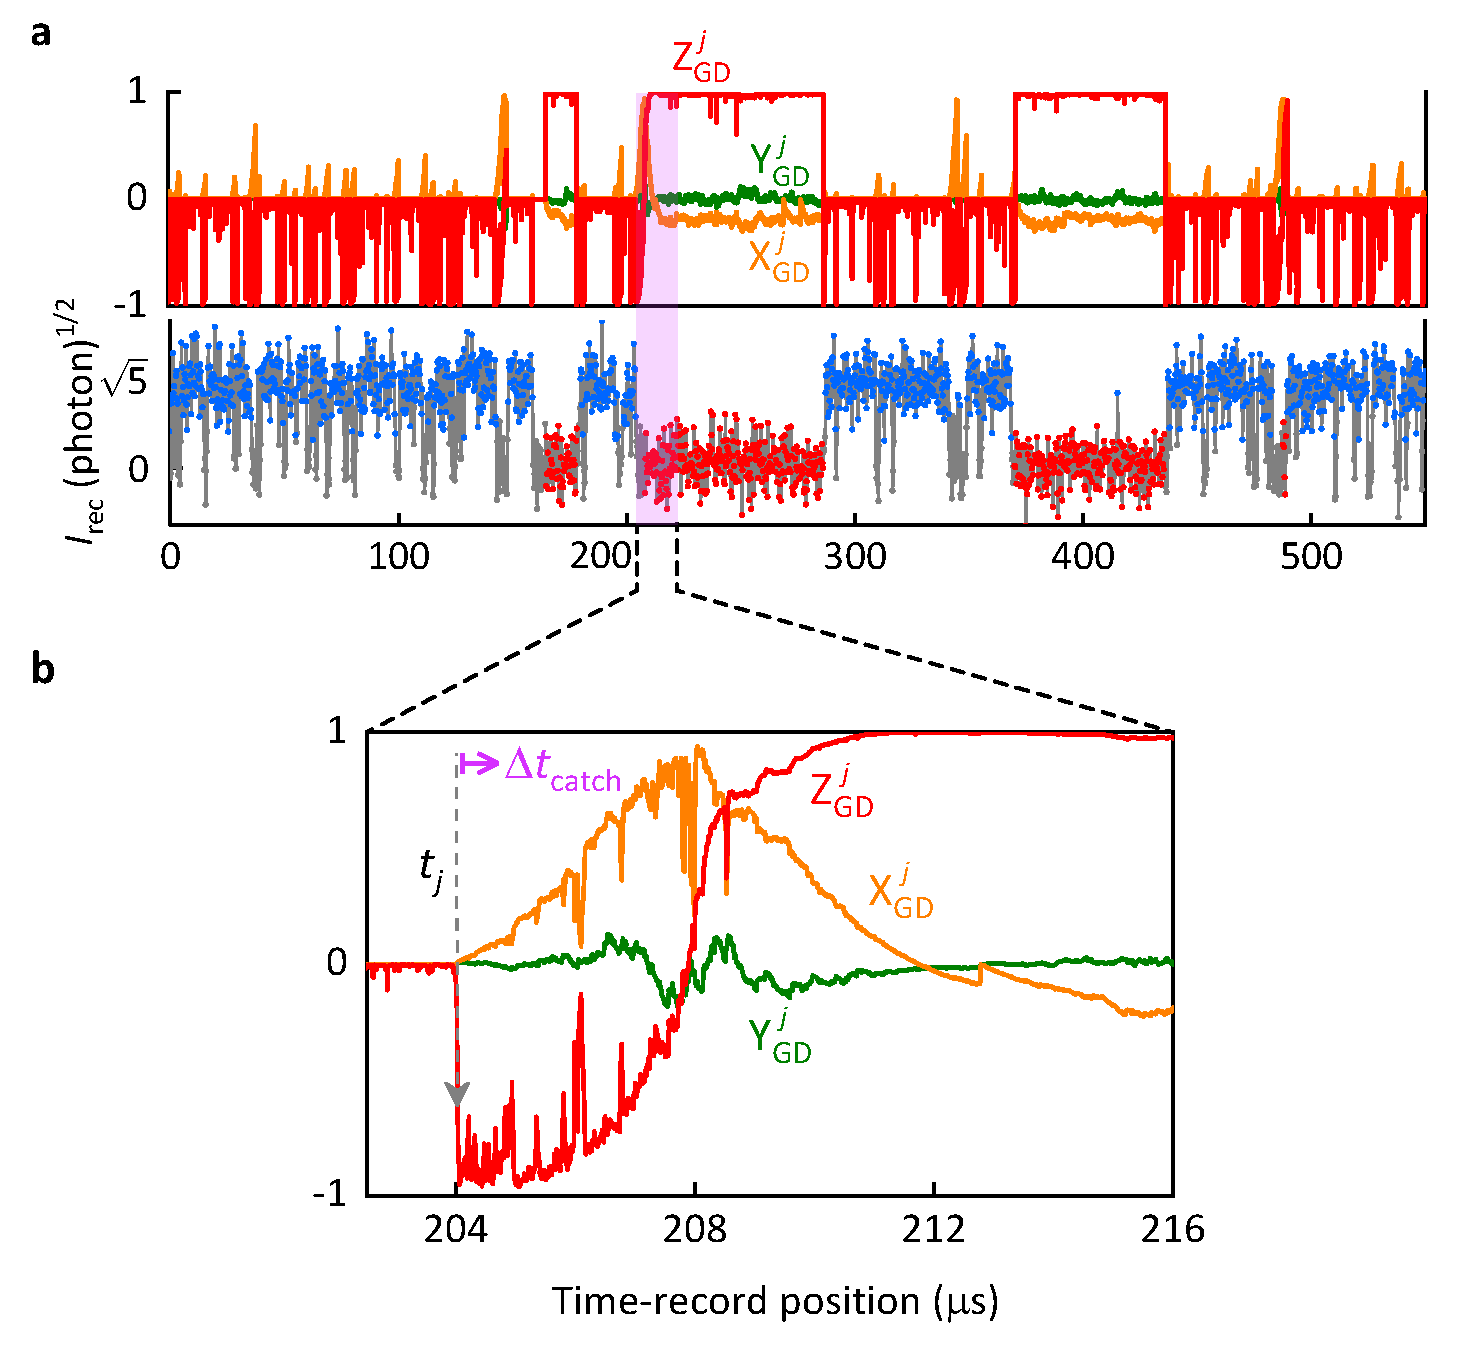
\includegraphics[width=145mm]{results/SamplingMC}\caption[Sampling of the Monte-Carlo simulation (courtesy of H.J. Carmichael)]{\label{fig:monte-carlo} \textbf{Sampling of the Monte-Carlo simulation.}
\textbf{a,} Simulated measurement quadrature $I_{{\rm rec}}$ and
correlated trajectory computed from Eqs.~(\ref{eqn:correlated_Z_GD})
and (\ref{eqn:correlated_X_GD=000026Y_GD}). Three sample intervals
are shown. The earliest corresponds to leakage from the GBD-manifold,
where a jump from $|{\rm G}\rangle$ to $|{\rm F}\rangle$ is followed
by a jump from $|{\rm F}\rangle$ to $|{\rm D}\rangle$. The second
and third sample intervals correspond to direct transitions from $|{\rm G}\rangle$
to $|{\rm D}\rangle$, which are continuously monitored and the object
of the experiment. \textbf{b,} Expanded view of the shaded region
of the second sample interval in panel (a). The evolution is continuous
but not smooth, due to backaction noise from the continuously monitored
readout. This feature is in sharp contrast to the perfect ``no-click''
readout upon which the simple theory of Sec.~\ref{sec:Fluorescence-monitored-by}
is based. Figure courtesy of H.J. Carmichael.}
\end{figure}

\begin{figure}
\centering{}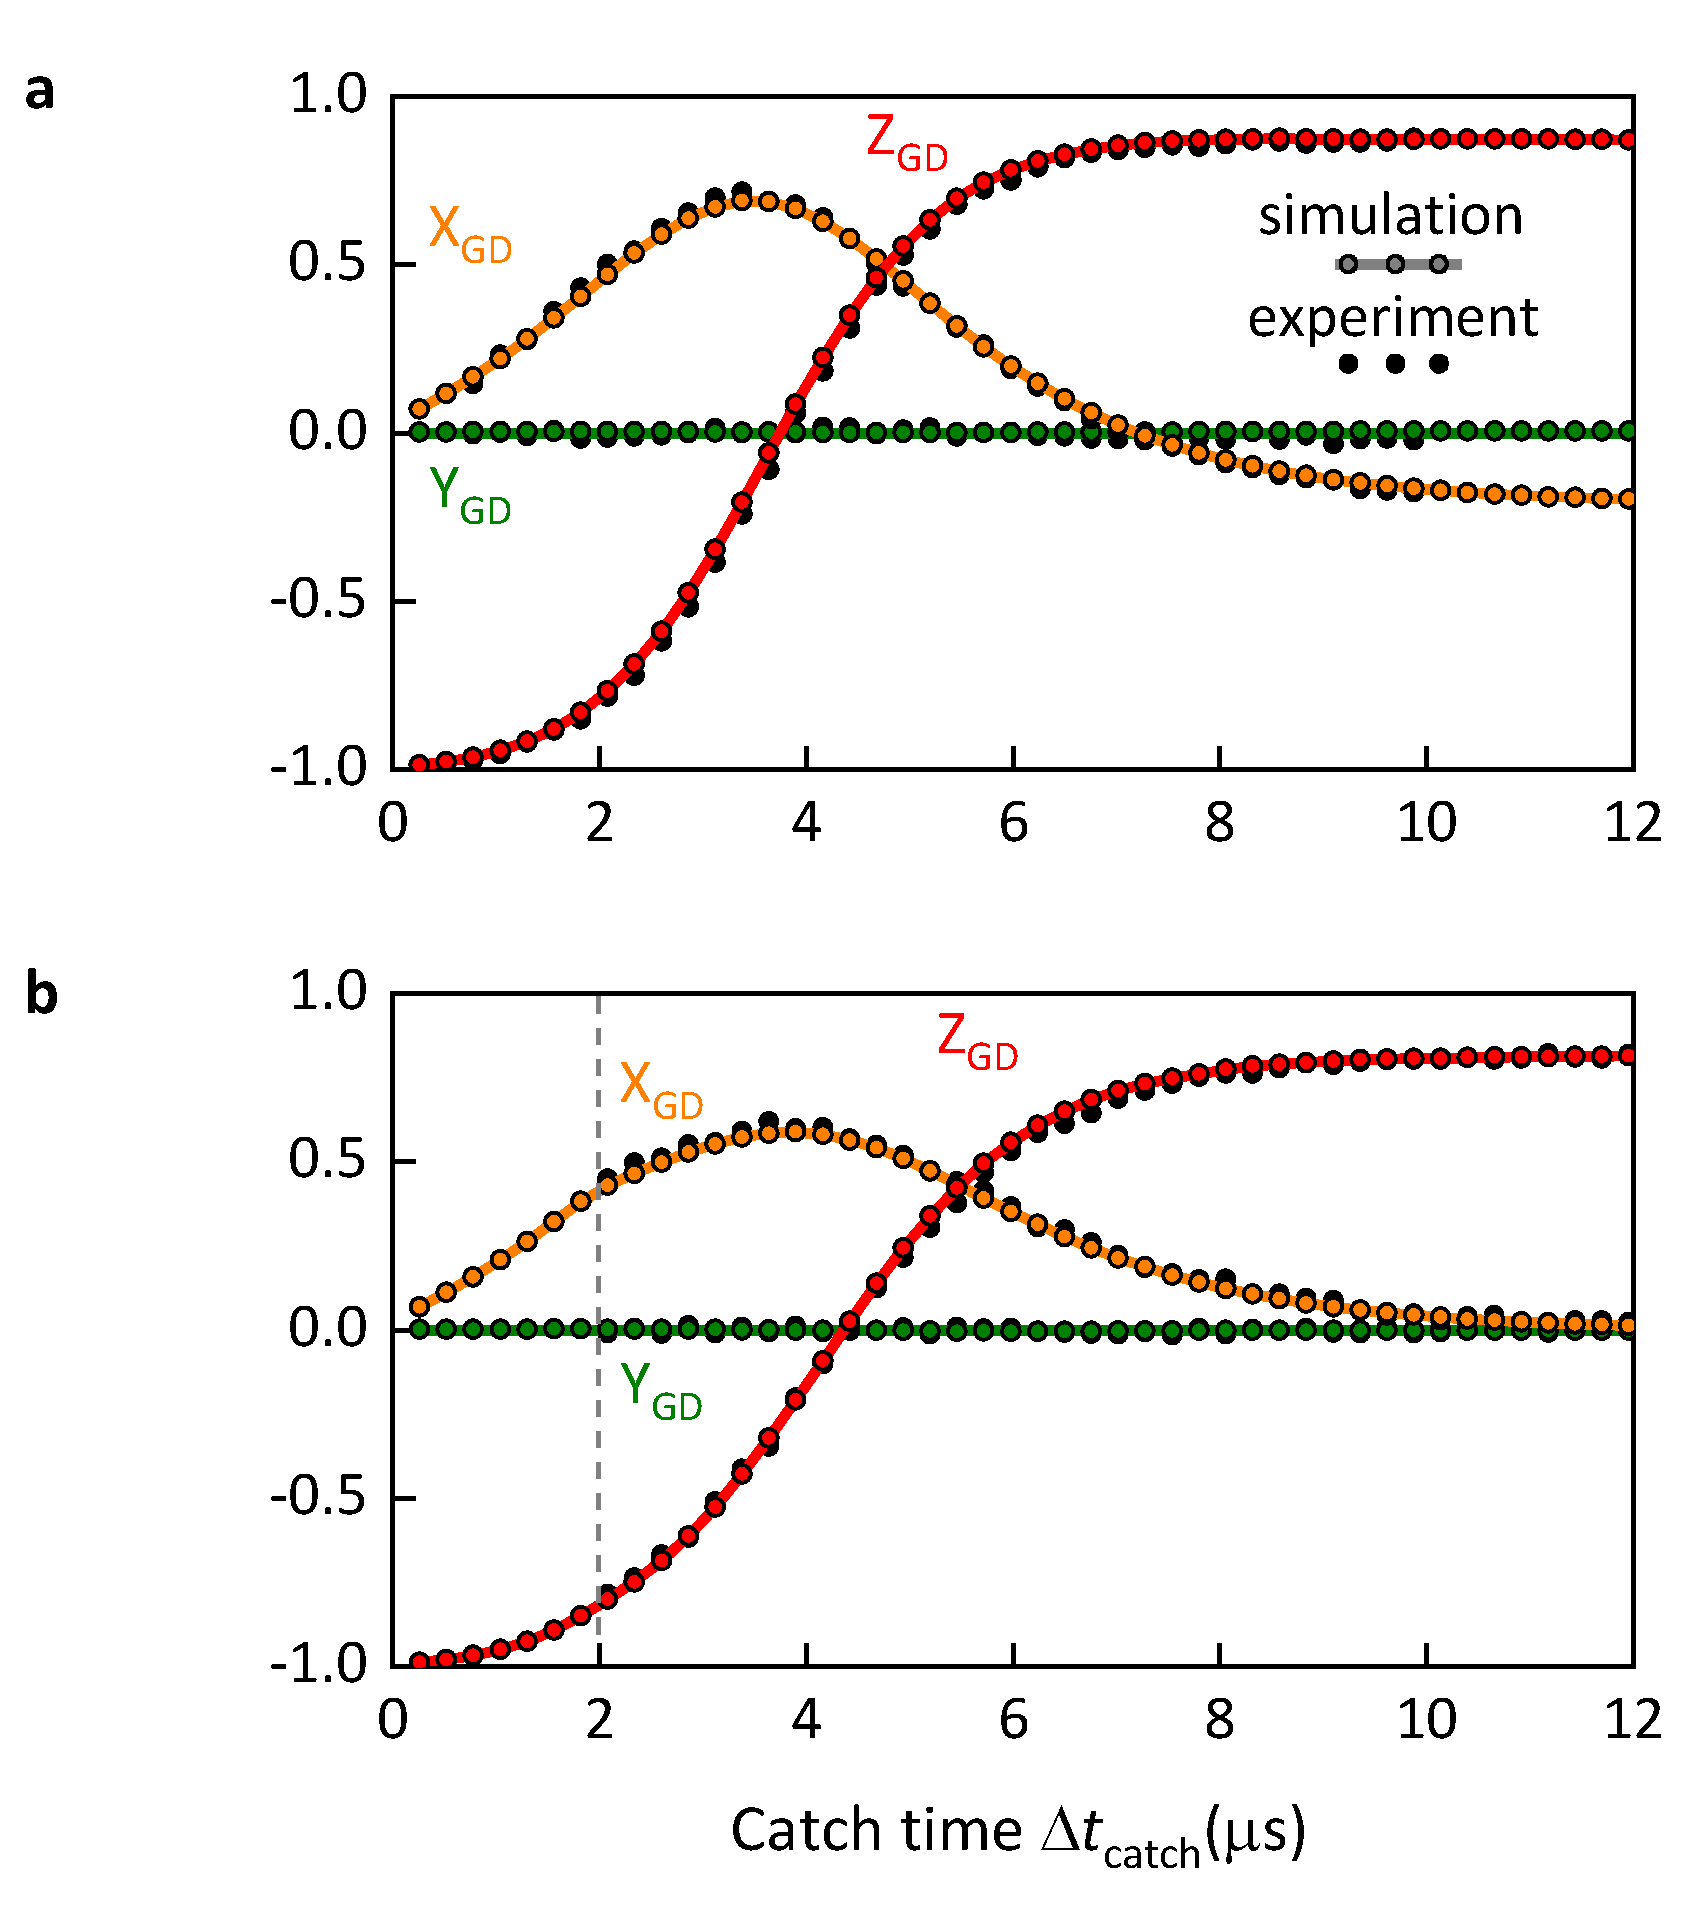
\includegraphics[width=120mm]{results/tomoCompar}\caption[Comparison between simulation and experiment (courtesy of H.J. Carmichael)]{\label{fig:simulation_vs_experiment} \textbf{Comparison between
simulation and experiment.} \textbf{a,} Simulated data set obtained
with Rabi drive $\Omega_{{\rm DG}}$ turned on for the entire $\Delta t_{{\rm catch}}$;
parameters taken from Table \ref{table:table2} and leakage from the
GBD-manifold included with $(\gamma_{{\rm FG}},\gamma_{{\rm FD}})/2\pi=0.38\mkern2mu {\rm kHz}$
and $(\gamma_{{\rm GF}},\gamma_{{\rm DF}})/2\pi=11.24\mkern2mu {\rm kHz}$.
\textbf{b,} Simulated data set obtained with Rabi drive $\Omega_{{\rm DG}}$
turned off at time $\Delta t_{{\rm on}}=2\mkern2mu \mu{\rm s}$; parameters
taken from Table \ref{table:table2} and leakage from the GBD-manifold
included with $\gamma_{{\rm FG}}/2\pi=0.217\mkern2mu {\rm kHz}$,
$\gamma_{{\rm FD}}/2\pi=4.34\mkern2mu {\rm kHz}$, $\gamma_{{\rm GF}}/2\pi=11.08\mkern2mu {\rm kHz}$,
and $\gamma_{{\rm DF}}/2\pi=15.88\mkern2mu {\rm kHz}$. When leakage
from the GBD-manifold is omitted, the ${\rm Z}_{{\rm GD}}$ curve
rises more sharply and settles to a value that is 10\% (20\%) higher
in panel (a) (panel (b)). Figure courtesy of H.J. Carmichael.}
\end{figure}

\clearpage{}

\begin{table}
\begin{centering}
\begin{tabular}{c}
\textbf{(a)} In presence of $\Omega_{\mathrm{DG}}$\tabularnewline
\tabularnewline
\centering{}\renewcommand*{\arraystretch}{1.2} %
\begin{tabular}{cc|crcllrrlcr}
Parameter  & \multicolumn{1}{c|}{} &  & \multicolumn{3}{c}{Experiment} &  & \multicolumn{3}{c}{Simulation} &  & Error\tabularnewline
\hline 
\rule{0pt}{3ex} $a$  &  &  & -0.07  & $\pm$  & 0.005  &  & -0.07  & $\pm$  & 0.005  &  & 0.5\%\tabularnewline
$a'$  &  &  & -0.21  & $\pm$  & 0.005  &  & -0.22  & $\pm$  & 0.005  &  & 2\%\tabularnewline
$b$  &  &  & 0.94  & $\pm$  & 0.005  &  & 0.95  & $\pm$  & 0.005  &  & 1\%\tabularnewline
$b'$  &  &  & 0.93  & $\pm$  & 0.005  &  & 0.91  & $\pm$  & 0.005  &  & 2\%\tabularnewline
$c$  &  &  & -2.32  & $\pm$  & 0.03  &  & -2.27  & $\pm$  & 0.03  &  & 2\%\tabularnewline
$c'$  &  &  & -2.04  & $\pm$  & 0.03  &  & -2.05  & $\pm$  & 0.03  &  & 0.5\%\tabularnewline
$\tau$  &  &  & 1.64  & $\pm$  & 0.01  &  & 1.65  & $\pm$  & 0.01  &  & 0.5\%\tabularnewline
$\tau'$  &  &  & 1.74  & $\pm$  & 0.01  &  & 1.76  & $\pm$  & 0.01  &  & 1\%\tabularnewline
\end{tabular}\tabularnewline
\tabularnewline
\textbf{(b)} In absence of $\Omega_{\mathrm{DG}}$\tabularnewline
\tabularnewline
\centering{}\renewcommand*{\arraystretch}{1.2} %
\begin{tabular}{cc|crcllrrlcr}
Parameter & \multicolumn{1}{c|}{} &  & \multicolumn{3}{c}{Experiment} &  & \multicolumn{3}{c}{Simulation} &  & Error\tabularnewline
\hline 
\rule{0pt}{3ex} $a$ &  &  & -0.11 & $\pm$ & 0.005 &  & -0.10 & $\pm$ & 0.005 &  & 8\%\tabularnewline
$a'$ &  &  & 0 & $\pm$ & 0 &  & 0 & $\pm$ & 0 &  & 0\%\tabularnewline
$b$ &  &  & 0.92 & $\pm$ & 0.008 &  & 0.91 & $\pm$ & 0.008 &  & 1\%\tabularnewline
$b'$ &  &  & 0.61 & $\pm$ & 0.005 &  & 0.60 & $\pm$ & 0.005 &  & 2\%\tabularnewline
$c$ &  &  & -1.96 & $\pm$ & 0.05 &  & -2.10 & $\pm$ & 0.05 &  & 7\%\tabularnewline
$c'$ &  &  & -1.97 & $\pm$ & 0.05 &  & -2.05 & $\pm$ & 0.05 &  & 4\%\tabularnewline
$\tau$ &  &  & 2.17 & $\pm$ & 0.05 &  & 2.03 & $\pm$ & 0.05 &  & 6\%\tabularnewline
$\tau'$ &  &  & 1.98 & $\pm$ & 0.05 &  & 1.92 & $\pm$ & 0.05 &  & 3\%\tabularnewline
\end{tabular}\tabularnewline
\tabularnewline
\end{tabular}
\par\end{centering}
\caption[Comparison between parameters extracted from the simulation and those
from the experiment. ]{\label{tab:Comparison-of-parameters} \textbf{Comparison between
parameters extracted from the simulation and those from the experiment}.
\textbf{a,} Parameters obtained from fits of the simulated and measured
data for the catch protocol in the presence of the Rabi drive $\Omega_{{\rm DG}}$
throughout the entire duration of the quantum jump, data shown in
Fig.~\ref{fig:simulation_vs_experiment}a. \textbf{b,} Parameters
obtained from fits of the simulated and measured data for the catch
protocol in the absence of the $\Omega_{{\rm DG}}$ during the flight
of the quantum jump for $\Delta t_{\mathrm{on}}=2\mathrm{\ \mu s}$,
data shown in Fig.~\ref{fig:simulation_vs_experiment}b. }
\end{table}

\clearpage{}

\subsection{Error budget\label{sec:Budget-coherence}}

In this section, we examine the effect of the various imperfections
and dissipation channels on the fidelity of the catch protocol. 

\paragraph{\textit{\emph{Imperfections.}}}

The various imperfections are expected to reduce the maximum coherence
recovered in the measurement of ${\rm X}_{{\rm GD}}(\Delta t_{{\rm catch}})$.
They include: 
\begin{enumerate}
\item Readout errors when inferring $|{\rm B}\rangle$ to not-$|{\rm B}\rangle$
transitions and the reverse. Such errors affect the assignment of
$\Delta t_{{\rm catch}}$, which can be either too short or too long
to correlate correctly with the true state of the system. 
\item Leaks from the GBD-manifold to higher excited states. Importantly,
these errors mimic a $|{\rm B}\rangle$ to not-$|{\rm B}\rangle$
transition, as in the first sample interval of Fig.~\ref{fig:monte-carlo},
but the anticipated coherent evolution within the GBD-manifold does
not occur. In this manner, the excitations to higher states lead to
false detections.
\item Thermal jumps from $|{\rm G}\rangle$ to $|{\rm D}\rangle$. Such
incoherent transitions contribute in a similar way to ${\rm Z}_{{\rm GD}}(\Delta t_{{\rm catch}})$,
while making no contribution to the measured coherence. 
\item Direct dephasing of the DG-coherence, $T_{\mathrm{2R}}^{\mathrm{D}}$. 
\item Partial distinguishability of $|{\rm G}\rangle$ and $|{\rm D}\rangle$.
The readout cavity is not entirely empty of photons when the state
is not-$|{\rm B}\rangle$, in which case the cross-Kerr interaction
$\chi_{{\rm D}}|{\rm D}\rangle\langle{\rm D}|\hat{c}^{\dagger}\hat{c}$
shifts the $\Omega_{{\rm DG}}$ Rabi drive from resonance; hence,
backaction noise is transferred from the photon number to ${\rm X_{{\rm GD}}}(\Delta t_{{\rm catch}})$. 
\end{enumerate}

\paragraph{\textit{\emph{Budget for lost coherence.}}\emph{ }}

The maximum coherence reported in the experiment is $0.71\pm0.005$.
In the simulation it is a little lower at 0.69. By removing the imperfections
from the simulation, one by one, we can assign a fraction of the total
coherence loss to each. Readout errors are eliminated by identifying
transitions between $|{\rm B}\rangle$ and not-$|{\rm B}\rangle$
in the ket $|\psi\rangle$ rather than from the simulated measurement
record; all other imperfections are turned off by setting some parameter
to zero. The largest coherence loss comes from readout errors, whose
elimination raises the ${\rm X}_{{\rm GD}}(\Delta t_{{\rm catch}})$
maximum by 0.09. The next largest comes from leakage to higher excited
states, which raises the maximum by a further 0.06. Setting $\chi_{{\rm D}}$
to zero adds a further 0.04, and thermal transitions and pure dephasing
together add 0.02. Figure~\ref{fig:coherence_loss} illustrates the
change in the distribution of ${\rm X}_{{\rm GD}}^{j}(\Delta t_{{\rm catch}})$
samples underlying the recovery of coherence. The removal of the finger
pointing to the left in panel (a) is mainly brought about by the elimination
of readout errors, while the reduced line of zero coherence marks
the elimination of leakage to higher excited states. Aside from these
two largest changes, there is also a sharpening of the distribution,
at a given $\Delta t_{{\rm catch}}$, when moving from panel (a) to
panel (b). Having addressed the five listed imperfections, a further
10\% loss remains unaccounted for, i.e., the distribution of panel
(b) is not a line passing through ${\rm X}_{{\rm GD}}^{j}(\Delta t_{{\rm mid}})=1$.
The final 10\% is explained by the heterodyne detection backaction
noise, a function of the drive and measurement parameters, displayed
in panel (b) of Fig.~\ref{fig:monte-carlo}. 
\begin{figure}[h]
\begin{centering}
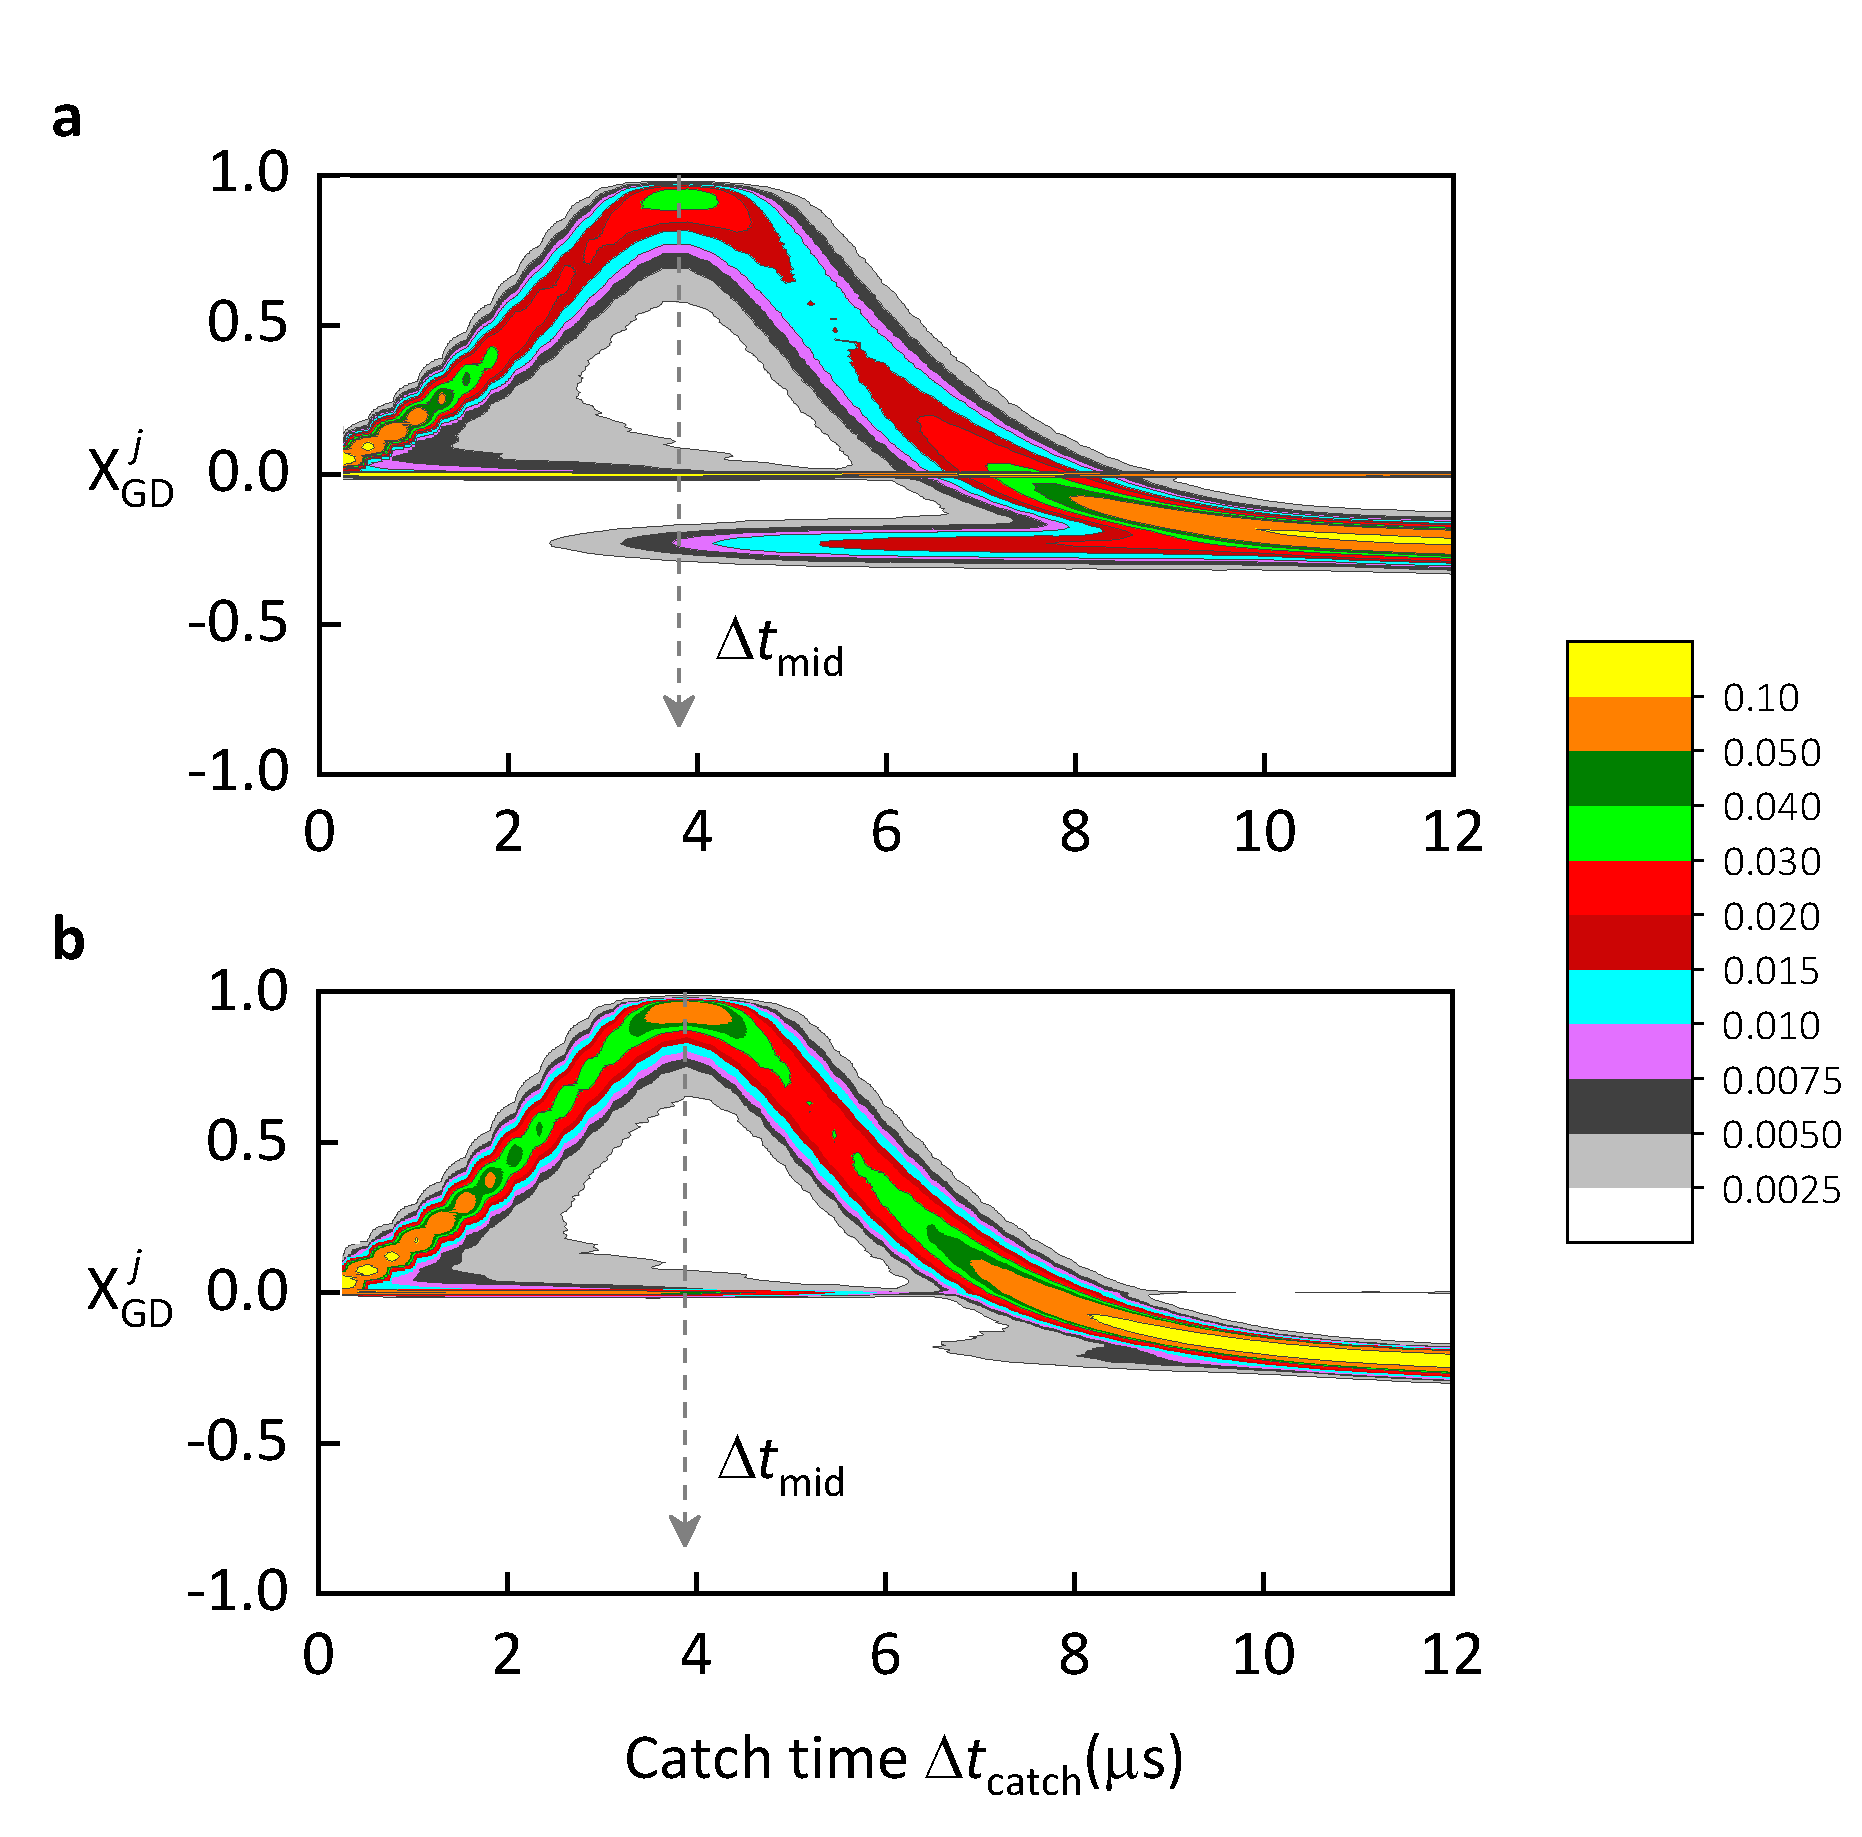
\includegraphics[width=130mm]{results/traj_hist}
\par\end{centering}
\centering{}\caption[Coherence loss through sample to sample fluctuations (courtesy of
H.J. Carmichael)]{\label{fig:coherence_loss}\textbf{Coherence loss through sample
to sample fluctuations.} \textbf{a,} Contour plot of the distribution
of ${\rm X}_{{\rm GD}}^{j}(\Delta t_{{\rm catch}})$ samples corresponding
to the simulated data set displayed in panel (a) of Fig.~\ref{fig:simulation_vs_experiment}.
\textbf{b,} Same as panel (a) but with transitions between $|{\rm B}\rangle$
and not-$|{\rm B}\rangle$ identified in the ket $|\psi\rangle$ rather
than from the simulated measurement record, and with changed parameters:
$(\gamma_{{\rm FG}},\gamma_{{\rm FD}},\gamma_{{\rm GF}},\gamma_{{\rm DF}})/2\pi=0$,
$n_{{\rm th}}^{{\rm B}}=n_{{\rm th}}^{{\rm D}}=0$, $T_{2}^{{\rm D}}=2T_{1}^{{\rm D}}$,
and $\chi_{{\rm D}}/2\pi=0$. Figure courtesy of H.J. Carmichael.}
\end{figure}


\section{Signal-to-noise ratio (SNR) and de-excitation measurement efficiency\label{subsec:Signal-to-noise-ratio-(SNR)}}

The catch protocol hinges on the efficient detection of de-excitations
from $|{\rm B}\rangle$ to $|{\rm G}\rangle$, as discussed in more
detail in Chapter~\ref{chap:theoretical-description-jumps}. In atomic
physics, de-excitations are typically monitored by a \emph{direct}
detection method, employing a photodetector. Alternatively, de-excitations
can be monitored by an\emph{ indirect} method, as done in our experiment.
In this section, we discuss the efficiency of both methods. For the
indirect method, using simple analytics, we estimate the \emph{total}
efficiency of time-continuous, uninterrupted monitoring of de-excitations
from $|{\rm B}\rangle$ to $|{\rm G}\rangle$ to be $\eta_{\mathrm{eff,clk}}=0.90\pm0.01$
for the parameters of our experiment, with integration time $T_{\mathrm{int}}=0.26\,\mathrm{\mu s}$.
The simple analysis of this section complements the numerical one
of the previous section, Sec.~\ref{sec:Budget-coherence}.

\emph{Direct monitoring method in atomic physics.} The direct method
monitors for a $|{\rm B}\rangle$ de-excitation by collecting and
absorbing the photon radiated in the de-excitation. The \emph{total}
measurement efficiency of this method is limited by i) collection
efficiency --- the fraction of emitted photons collected by the detector
in its own input spatial modes (for instance, as determined by the
solid angle) --- typically falls in the range 0.1 - 50\%, \citep{Volz2011}
ii) the efficiency of detecting the absorption of a single photon,
which falls in the range 1 - 90\%, \citep{Eisaman2011} and iii) non-idealities
of the photodetector apparatus, including its dead time, dark counts,
jitter, etc. \citep{Eisaman2011} The combination of these inefficiencies
presents an almost insurmountable challenge in experimental atomic
physics for realizing continuous, time-resolved detection of nearly
every single photon emitted by the three-level atom, required to faithfully
catch the jump. 

\emph{Direct monitoring method with superconducting circuits.} While
technologically very different, the direct monitoring method with
superconducting circuits is conceptually similar to atomic method
but can readily achieve high collection efficiencies \citep{Katz2008,Vijay2011,Riste2012-qubit-measure-reset,Vijay2012,Hatridge2013,Murch2013a,deLange2014,Roch2014,Weber2014,Campagne-Ibarcq2014,Macklin2015,Campagne2016-Fluorescence,Campagne-Ibarcq2016,Hacohen-Gourgy2016-non-comm,Naghiloo2016,White2016,Ficheux2017,Naghiloo2017-thermo,Tan2017,Hacohen-Gourgy2018,Heinsoo2018,Bultink2018}.
 However, the energy of the emitted microwave photon is exceedingly
small --- $23\text{ }\mathrm{\mu eV}$, about a part per 100,000
of the energy of a single optical photon --- which essentially forbids
the direct detection of the photon with near-unit efficiency. This
is because the propagating photon is unavoidably subjected to significant
loss, added spurious noise, amplifier non-idealities, etc. In our
experiment, these imperfections reduce the full measurement/amplification
chain efficiency from its ideal value \citep{Hatridge2013,Macklin2015,Bultink2018}
of 1 to a modest $\eta=0.33\pm0.03$, corresponding to the direct
detection of approximately only one out of every three single photons
--- insufficient for the catch protocol.

\subsubsection{Indirect monitoring method with superconducting circuits}

Alternatively, the indirect monitoring method couples the atom to
an ancillary degree of freedom, which is itself monitored in place
of the atom. In our experiment, the atom is strongly, dispersively
coupled to the ancillary readout cavity. The cavity scatters a probe
tone, whose phase shift constitutes the readout signal, as discussed
in Chapter~\ref{chap:theoretical-description-jumps}. Since the probe
tone can carry itself many photons, this scheme increases the signal-to-noise
ratio ($\mathrm{SNR}$) and, hence, the total efficiency ($\eta_{\mathrm{eff,clk}}$)
of detecting a $|{\rm B}\rangle$ de-excitation. Note that the efficiency
$\eta_{\mathrm{eff,clk}}$ should not be confused with the efficiency
of a photodetector or the efficiency $\eta$ of the measurement/amplification
chain, since $\eta_{\mathrm{eff,clk}}$ includes the effect of all
readout imperfections and non-idealities, state discrimination and
assignment errors, etc. see below. In the remainder of this section,
we estimate the SNR and efficiency $\eta_{\mathrm{eff,clk}}$ of the
experiment.

\emph{SNR of the indirect (dispersive) method.}  The output of the
measurement and amplification chain monitoring the readout cavity
is proportional to the complex heterodyne measurement record $\zeta\left(t\right)$,
which obeys the It\^{o} stochastic differential equation, see Eq.~(\ref{eq:Record}),\footnote{Since the bandwidth of the measurement chain, $\kappa_{\mathrm{filter}}$,
is significantly larger than that, $\kappa$, of the readout cavity,
$\kappa_{\mathrm{filter}}\gg\kappa$, we can neglect the effect of
$\kappa_{\mathrm{filter}}$ for simplicity of discussion, see Eqs.~(\ref{eqn:simulated_I_int})
and~(\ref{eqn:simulated_Q_int}).} 
\begin{equation}
\mathrm{d}\zeta\left(t\right)=\sqrt{\eta\kappa}\frac{\langle\psi\left(t\right)|\hat{a}|\psi\left(t\right)\rangle}{\langle\psi\left(t\right)|\psi\left(t\right)\rangle}\mathrm{d}t+\mathrm{d}Z\left(t\right),\label{eq:heterodyne-current2}
\end{equation}
where $\hat{a}$ is the cavity amplitude operator in the Schr\"{o}dinger
picture, $\eta$ is the total measurement efficiency of the amplification
chain --- again, not to be confused with the de-excitation measurement
efficiency, $\eta_{\mathrm{eff,clk}}$ --- and $\mathrm{d}Z$ is
the complex Wiener process increment, defined below Eq.~(\ref{eq:heterodyne-current2}).
A somewhat counterintuitive property of Eq.~(\ref{eq:heterodyne-current2})
is that  the heterodyne record increment $\mathrm{d}\zeta\left(t\right)$
is stochastic and noisy even when $\eta=1$, the case of ideal measurement
in which no signal is lost --- the stochastic term, $\mathrm{d}Z$,
represents pure quantum vacuum fluctuations, which are inherent in
the case of heterodyne detection \citep{Carmichael1993,Plenio1998,wiseman2010book}.
Due to the unavoidable presence of these fluctuations, only an infinitesimal
amount of information about the system can be extracted from $\mathrm{d}\zeta$
at an instant of time. Finite amount of information is extracted by
integrating $\mathrm{d}\zeta$ for a finite duration $T_{\mathrm{int}}$,
\begin{equation}
s\equiv I_{\mathrm{rec}}+iQ_{\mathrm{rec}}\equiv\int_{0}^{T_{\mathrm{int}}}\mathrm{d}\zeta\left(t\right)\,,\label{eq:s=00003D}
\end{equation}
where $I_{\mathrm{rec}}$ and $Q_{\mathrm{rec}}$ are the in- and
out-of-phase quadrature components of one segment of the record. What
does $s$ correspond to? Its value depends on $\mathrm{d}\zeta$,
which depends on the state of the cavity, $|\psi\rangle$, which itself
depends on the occupation of $\ket{\mathrm{B}}$ --- and therefore
$s$ contains the occupation of $\ket{\mathrm{B}}$. A de-excitation
of $\ket{\mathrm{B}}$ to $\ket{\mathrm{G}}$ can thus be detected
by monitoring $s$, whose value is different for the two states, since
the cavity is generally in the coherent state $\ket{\alpha_{\mathrm{B}}}$
or $\ket{\alpha_{\mathrm{G}}}$ when the atom is in $\ket{\mathrm{B}}$
or $\ket{\mathrm{G}}$, respectively. For the moment, assuming the
atom and cavity do not change states during the course of the measurement
duration $T_{\mathrm{int}}$, the stochastic integral in Eq.~(\ref{eq:s=00003D})
explicitly evaluates to 
\begin{equation}
s_{\mathrm{B,G}}=\left\{ \sqrt{\eta\kappa}\mathrm{Re}\left[\alpha_{\mathrm{B,G}}\right]T_{\mathrm{int}}+\frac{1}{\sqrt{2}}W_{I}\left(T_{\mathrm{int}}\right)\right\} +i\left\{ -\sqrt{\eta\kappa}\mathrm{Im}\left[\alpha_{\mathrm{B,G}}\right]T_{\mathrm{int}}+\frac{1}{\sqrt{2}}W_{Q}\left(T_{\mathrm{int}}\right)\right\} \,,\label{eq:s=00003DExplicit}
\end{equation}
where $W_{I,Q}$ denote independent Wiener processes, obeying the
conventional rules, $\mathrm{E}\left[W\left(t\right)\right]=0$ and
$\mathrm{Var}\left[W\left(t\right)\right]=t^{2}$. Equation~(\ref{eq:s=00003DExplicit})
shows that the distribution of the stochastic variable $s$ is a Gaussian
blob in the IQ plane centered at $\bar{s}_{\mathrm{B,G}}\equiv\operatorname{E}\left[s_{\mathrm{B,G}}\right]=\sqrt{\eta\gamma}T_{\mathrm{int}}\alpha_{\mathrm{B,G}}$
with width determined by the variance $\sigma_{\mathrm{B,G}}^{2}\equiv\operatorname{Var}\left[s_{\mathrm{B,G}}\right]=\frac{1}{2}T_{\mathrm{int}}$.
We can thus define the SNR of the experiment by comparing the distance
between the two pointer distributions to their width, 
\begin{equation}
\mathrm{SNR}\equiv\left|\frac{\bar{s}_{\mathrm{B}}-\bar{s}_{\mathrm{G}}}{\sigma_{\mathrm{B}}+\sigma_{\mathrm{G}}}\right|^{2}\,,\label{eq:SNR-defn}
\end{equation}
where the B (resp., G) subscript denotes signals conditioned on the
atom being in $\ket{\mathrm{B}}$ (resp., $\ket{\mathrm{G}}$). In
terms of $\ket{\alpha_{\mathrm{B}}}$ and $\ket{\alpha_{\mathrm{G}}}$,
\begin{equation}
\mathrm{SNR}=\frac{1}{2}\eta\kappa T_{\mathrm{int}}\left|\alpha_{\mathrm{B}}-\alpha_{\mathrm{G}}\right|^{2}\,,
\end{equation}
which can be expressed in terms of the parameters of the experiment,
summarized in Table~\ref{tab:system-params},
\begin{equation}
\mathrm{SNR}=\frac{1}{2}\eta\kappa T_{\mathrm{int}}\left[\cos\left(\arctan\left(\frac{\kappa}{2\chi_{\mathrm{BG}}}\right)\right)\right]^{2}\bar{n}\,,\label{eq:SNR-expression}
\end{equation}
Holding other parameters fixed, according to Eq.~(\ref{eq:SNR-expression}),
the SNR can be increased arbitrarily by increasing $\bar{n}$, which
can be readily done by increasing the amplitude of the cavity probe
tone. A higher SNR for $s$ corresponds to a higher SNR for measuring
an atom de-excitation, since $s$ is a proxy of the $\ket{\mathrm{B}}$
population. Thus, the indirect cavity monitoring can overcome the
typical degradation in SNR imposed by the inefficiencies and non-idealities
of the measurement chain, $\eta$. In practice, the SNR increase
with $\bar{n}$ is bounded from above, since with sufficiently high
$\bar{n}$ spurious non-linear effects become significant \citep{Boissonneault2008,Boissonneault2009-Photon-induced-relax,Minev2013,Sank2016-T1vsNbar,Khezri2016,Bultink2016,Khezri2017,Walter2017,Lescanne2018,Verney2018,Serniak2018}.
The cavity and non-linear coupling to the atom serve in effect as
a rudimentary embedded pre-amplifier at the site of the atom, which
transduces with amplification the de-excitation signal before its
SNR is degraded during propagation and further processing.

\emph{Discrimination efficiency of the indirect method.} While the
SNR provides a basic characterization of the measurement, it is useful
to convert it to a number between 0 and 1, which is called the discrimination
efficiency, $\eta_{\mathrm{disc}}$. It quantifies the degree to which
the two Gaussian distributions of $s$ are distinguishable \citep{Gambetta2007-ProtocolsMsr},
\begin{equation}
\eta_{\mathrm{disc}}=\frac{1}{2}\operatorname{erfc}\left[-\sqrt{\frac{\mathrm{SNR}}{2}}\right]\,,\label{eq:eta-msr}
\end{equation}
where $\operatorname{erfc}$ denotes the complementary error function.
Equation~(\ref{eq:eta-msr}) shows that increasing the SNR by separating
the $s_{\mathrm{B}}$ and $s_{\mathrm{G}}$ distributions far beyond
their spread, $\sigma_{\mathrm{B/G}}$, provides only marginal gain
as $\eta_{\mathrm{disc}}$ saturates to 1. Next, we calculate the
SNR and $\eta_{\mathrm{disc}}$ for the parameters of the experiment
and discuss corrections due to readout non-idealities. 

\emph{A first comparison to the experiment. }A first estimate of the
SNR and $\eta_{\mathrm{disc}}$ of the experiment are provided by
Eqs.~(\ref{eq:SNR-expression}) and~(\ref{eq:eta-msr}). Using the
parameters of the experiment, summarized in Table~\ref{tab:system-params},
from these two equations, we find $\mathrm{SNR}=4.3\pm0.6$ and $\eta_{\mathrm{disc}}=0.98\pm0.007$.
Using data from the experiment, in particular, a second long IQ record
trace, represented by a short segment in Fig.~2a, we find the SNR
of the jumps experiment, by fitting the histogram of the trace with
a bi-Gaussian distribution, to be $\mathrm{SNR}=3.8\pm0.4$, corresponding
to $\eta_{\mathrm{\mathrm{disc}}}=0.96\pm0.01$. The measured values
are slightly lower than the analytics predict due to readout imperfections
not included in the calculation so far, such as state transitions
during $T_{\mathrm{int}}$, cavity transient dynamics, additional
pointer-state distributions, etc.

\emph{Effective click detection efficiency. }The dominant next-order
error is due to atom state transitions during the measurement window,
$T_{\mathrm{int}}$, which contributes an assignment error of approximately
$1-\eta_{\mathrm{asg}}=1-\exp\left(T_{\mathrm{int}}/\tau_{\mathrm{B}}\right)=0.06\pm0.001$
to the detection of a $|\mathrm{B}\rangle$ de-excitation. Combining
$\eta_{\mathrm{disc}}$ with $\eta_{\mathrm{asg}}$, we obtain the
total efficiency for detecting $\ket{\mathrm{B}}$ de-excitations
$\eta_{\mathrm{eff,clk}}=\eta_{\mathrm{disc}}\eta_{\mathrm{asg}}=0.90\pm0.01$,
consistent with the total readout efficiency of $0.91$ that is independently
estimated using the trajectory numerics, see Sec.~\ref{sec:Budget-coherence}.

